\section{Interaction Patterns Between Ase1 and Dynamic Microtubules}
\label{sec:Ase1}

\subsection{The effect of Ase1 on microtubule dynamic instability}
\label{sec:ase11}
\begin{figure}[h]
    \centering
    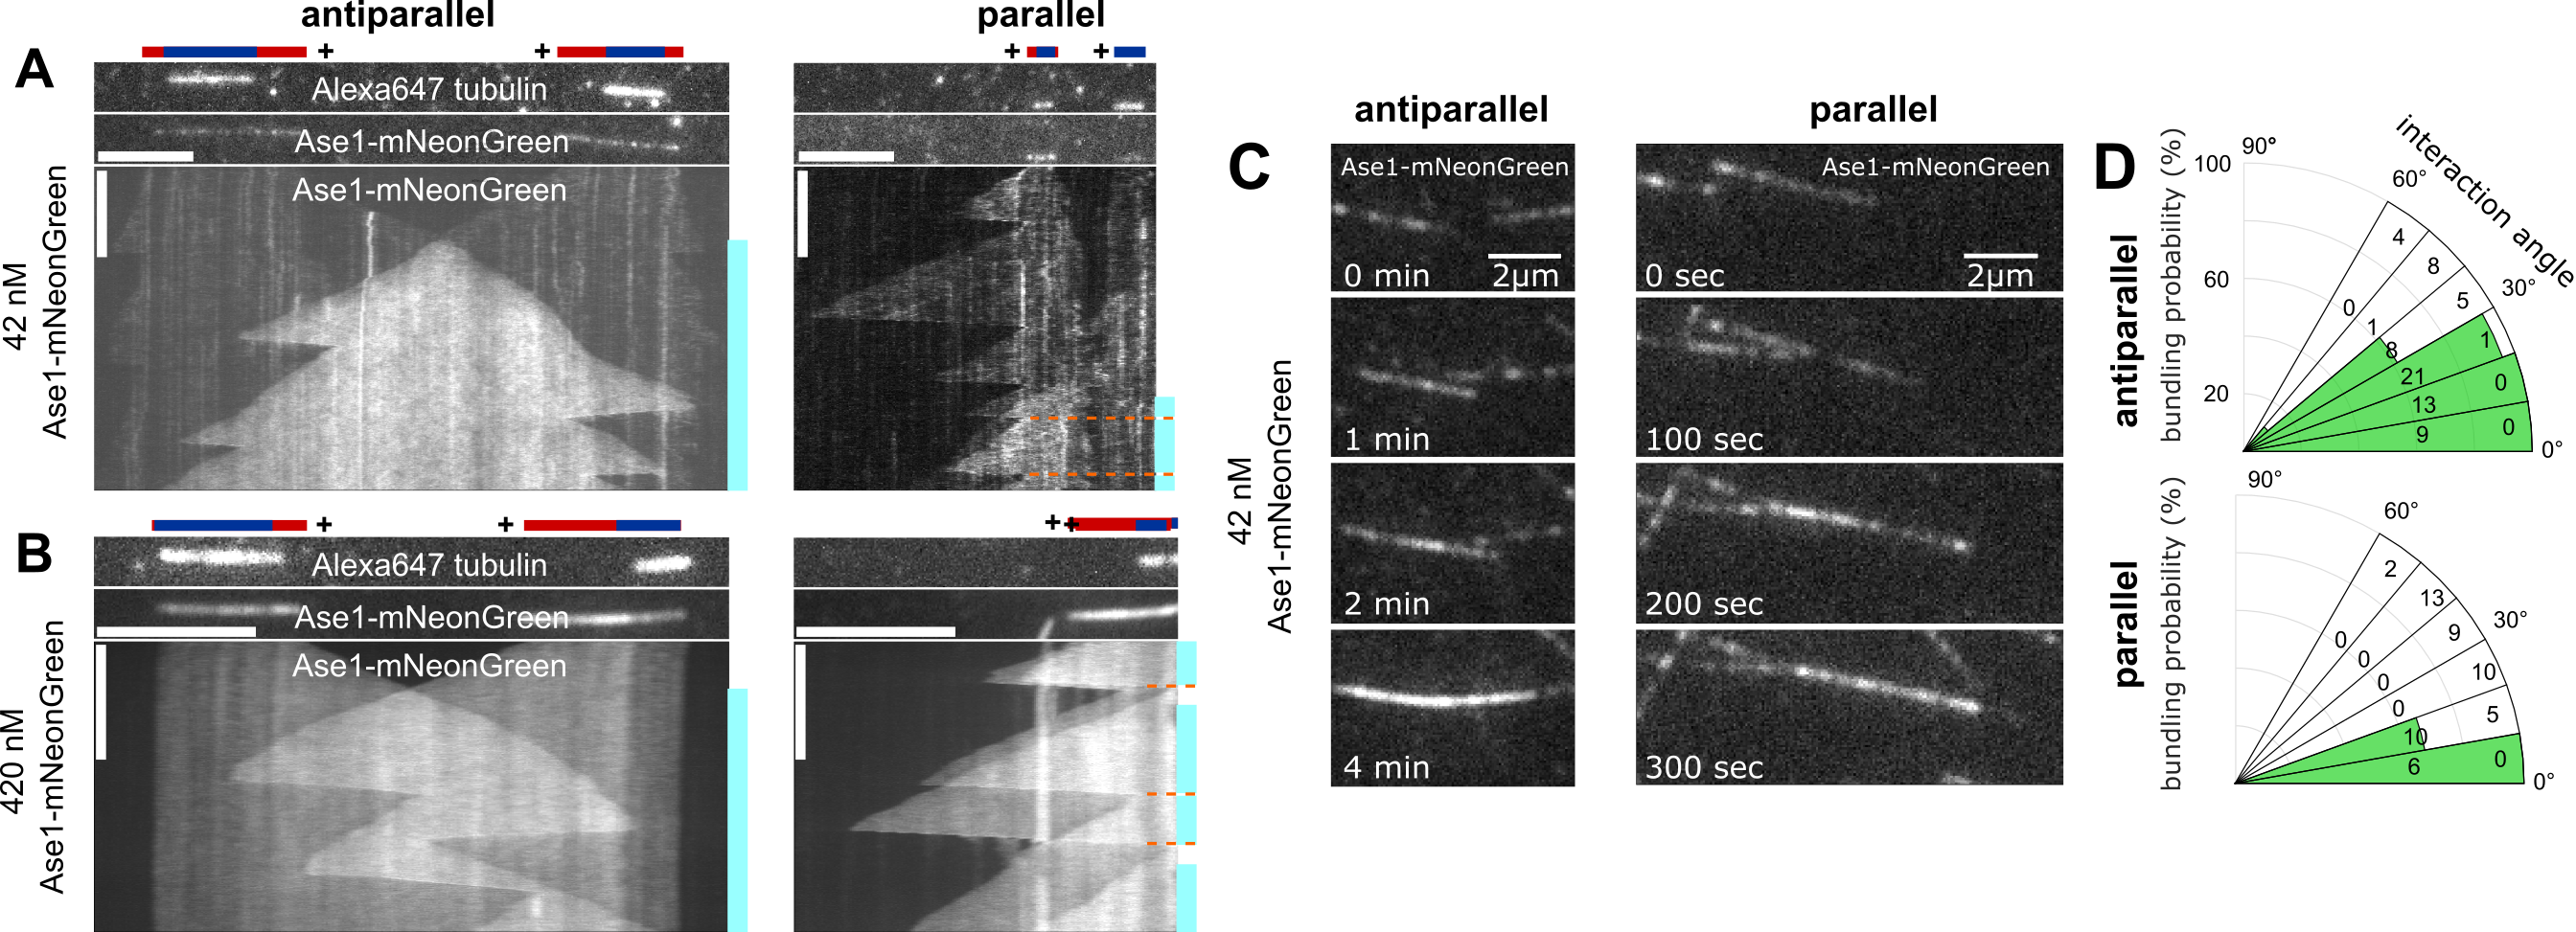
\includegraphics[width=1\linewidth]{Figures/ase1_1a.png}
    \caption[With dynamic microtubule extensions and Ase1, we observed microtubule bundling as previously reported.]{
    (A) Kymographs of an antiparallel (left panel) and a parallel microtubule overlap forming due to the microtubules polymerizing such to enable bundling by Ase1, which is present in solution (42nM). The scale bars are 5 micron and 10 minutes. In sketches, dynamic extensions with GDP lattices are red, and stabilized GMPCPP seeds are blue. The teal bars next to kymographs indicate the presence of regions of overlap (we only counted regions where the two partaking microtubule regions are constituted by GDP-tubulin, i.e., a seed stabilized by GMPCPP did not count). The orange lines indicate a termination of the overlapping period, as evaluated for \autoref{ase1b}A. (B) Same representation as A showing events from experiments performed at 420nM Ase1. (C) Snapshots of different events than shown in A and B, illustrating microtubule bundling (at 42nM). (D) Bundling probability for situations when microtubule plus ends encountered other microtubules, in either parallel or antiparallel orientation, versus the initial angle of interaction (results pooled for all Ase1-mNeonGreen concentrations). The outer numbers denote the numbers of recorded crossings at the respective angle, while the inner numbers denote the numbers of bundling events (the sum of both numbers is the total number of observed events). Panels taken from \cite{Krattenmacher2024}.
        }\label{ase1a}
\end{figure}
To investigate the interaction dynamics between diffusible microtubule crosslinkers and microtubules, we employed total internal reflection fluorescence (TIRF) and interference reflection microscopy (IRM) (\autoref{sec:microscopy}) time-lapse imaging of immobilized, GMPCPP-stabilized microtubule seeds in the presence of 30 µM free tubulin and varying concentrations of Ase1 (Methods). At concentrations of 42 nM and 420 nM Ase1, we observed dynamic, Ase1-decorated microtubule extensions polymerizing from the microtubule seeds \pref{ase1a}{A,B}. When two microtubule plus ends, emanating from different seeds and polymerizing towards each other, encountered each other, the microtubules either bundled or crossed, depending on the angle of incidence. Typically, at high angles, the microtubules crossed and only interacted at the crossing point, while at small angles, either parallel or antiparallel associations could be formed \pref{ase1a}{C}. As previously reported \parencite{Janson2007}, antiparallel bundles formed even at large initial angles of incidence (up to 40°), while parallel bundles only formed at initial angles below 20° \pref{ase1a}{D}.\par
\begin{wrapfigure}{l}{0.4\textwidth}
    \centering
    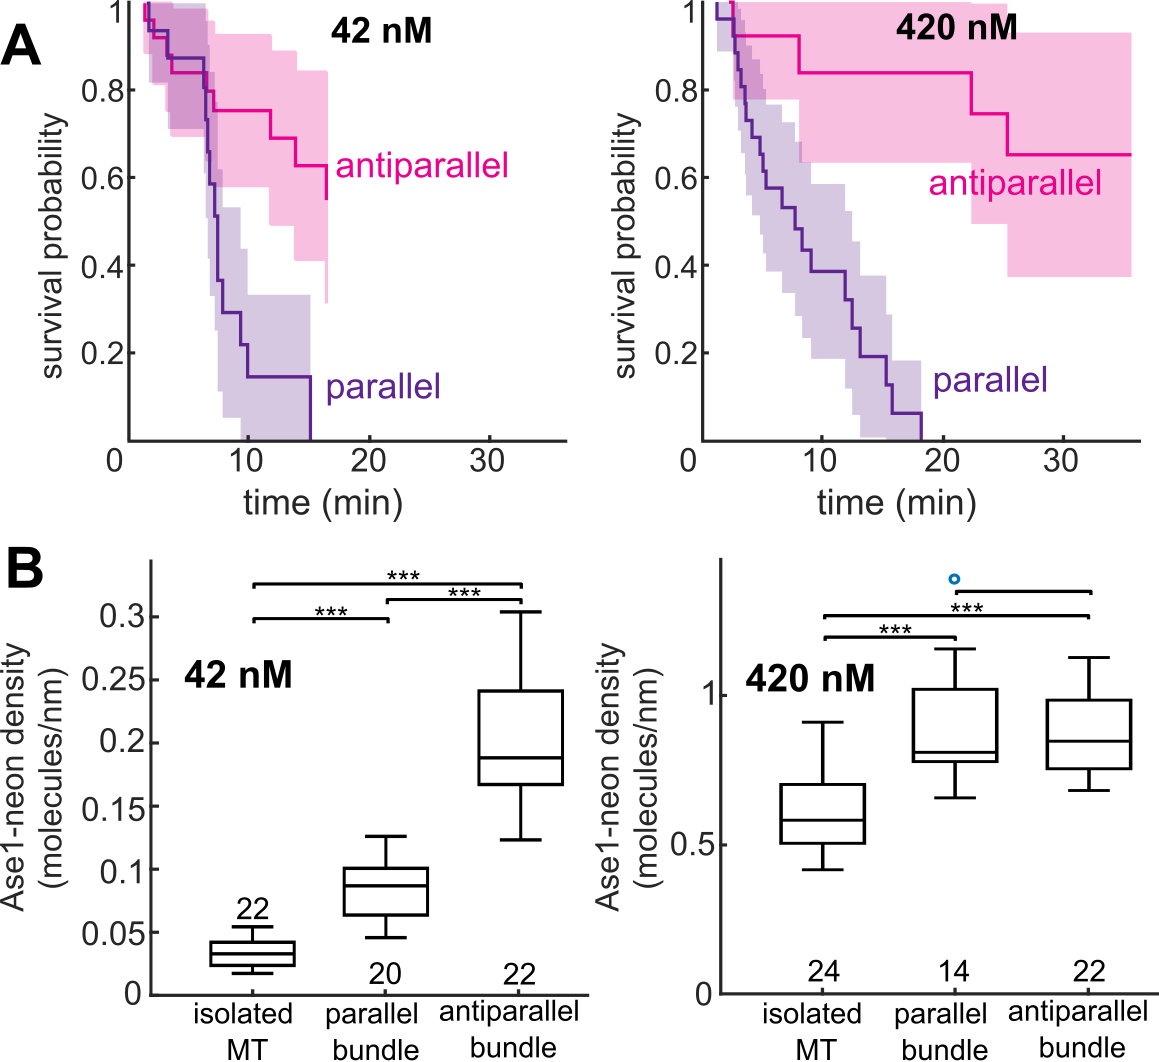
\includegraphics[width=1\linewidth]{Figures/ase1_1b.png}
    \caption[Ase1 selectively stabilizes antiparallel overlaps.]{
    (A) Survival probability of antiparallel and parallel overlaps, showing the probability that an overlap formed by two dynamic MT extensions persists at a given time after its formation (Methods). Semitransparent regions indicate 95\% lower and upper confidence bounds. (B) Quantification of the density of Ase1-mNeonGreen on isolated MTs and (anti)parallel bundles (Methods). The numbers below the boxes denote the number of analyzed microtubule bundles. Panels show data for MT plus ends (minus ends generally were not analyzed). Panels taken from \cite{Krattenmacher2024}.
        }\label{ase1b}
\end{wrapfigure}
Quantitative analysis revealed increased lifetimes of antiparallel overlaps compared to parallel ones\pref{ase1b}{A} Notably, at 42 nM Ase1 in solution, the Ase1 density on antiparallel overlaps was an order of magnitude higher than on parallel ones\pref{ase1b}{B} consistent with the previously reported differential affinities \parencite{Janson2007}. At 420 nM Ase1, we observed the density of Ase1 to be similar on antiparallel and parallel bundles, roughly twice the density found on isolated microtubules\pref{ase1b}{B} This possibly indicated that, at this high concentration, a similar number of Ase1 molecules was present within parallel and antiparallel overlaps. Note, however, that this value represents the total density of Ase1 at the bundle, which might differ from the density of Ase1 molecules directly engaged in MT crosslinking by being bound simultaneously to both microtubules. Despite similar decoration levels by Ase1, antiparallel overlaps were still significantly more stable than parallel ones\pref{ase1b}{A} Given the low polymerization velocity of minus ends, we very rarely observed antiparallel overlaps formed by two minus ends encountering each other, and we thus could not meaningfully quantify the associated lifetime. Generally, we chose to not analyze minus ends given that they are not dynamic \textit{in vivo} \parencite{dammer}.\par

To test whether the relative stability of antiparallel overlaps was caused by Ase1 crosslinking or the bundling itself (as was requested by a reviewer), we also conducted experiments at 10nM Ase1. At this concentration, we observed significantly less Ase1 within antiparallel bundles \pref{ase1c}{A}, and indeed, antiparallel bundles were no more stable than parallel bundles \pref{ase1c}{B}. Also, at 10nM Ase1 we observed antiparallel microtubules to no longer bundle as readily as at higher Ase1 concentrations \pref{ase1c}{C}. While we could detect an Ase1 signal at antiparallel overlaps, we did observe events where Ase1 crosslinking apparently was not strong enough to keep a MT plus end bundled to the MT along which it was growing in an antiparallel orientation \pref{ase1c}{D,E left panel}. Finally, to test whether microtubule bundling in our assays was partially a result of molecular crowding (and not Ase1), we performed an assay at 0nM Ase1. In absence of Ase1, microtubules never bundled, even when very close to each other over extended periods of time, indicating that molecular crowding did not play a role in the microtubule bundling we observed \pref{ase1c}{F}. \par

The relative stability of antiparallel overlaps at high Ase1 concentrations may at least partly owe to the fact that antiparallel overlaps grow with twice the speed of parallel overlaps (since both microtubules polymerize in opposite directions, however it should be noted that once a minus end has been surpassed the antiparallel overlaps does no longer grow as quickly on the side in question); hence, there is more opportunities for rescues to occur during depolymerization. However, our kymographs suggested that antiparallel overlaps may be additionally stabilized by an increase in rescue frequency \pref{ase1d}{A}, and we set out to quantify this issue next. \par

\begin{figure}[h]
    \centering
    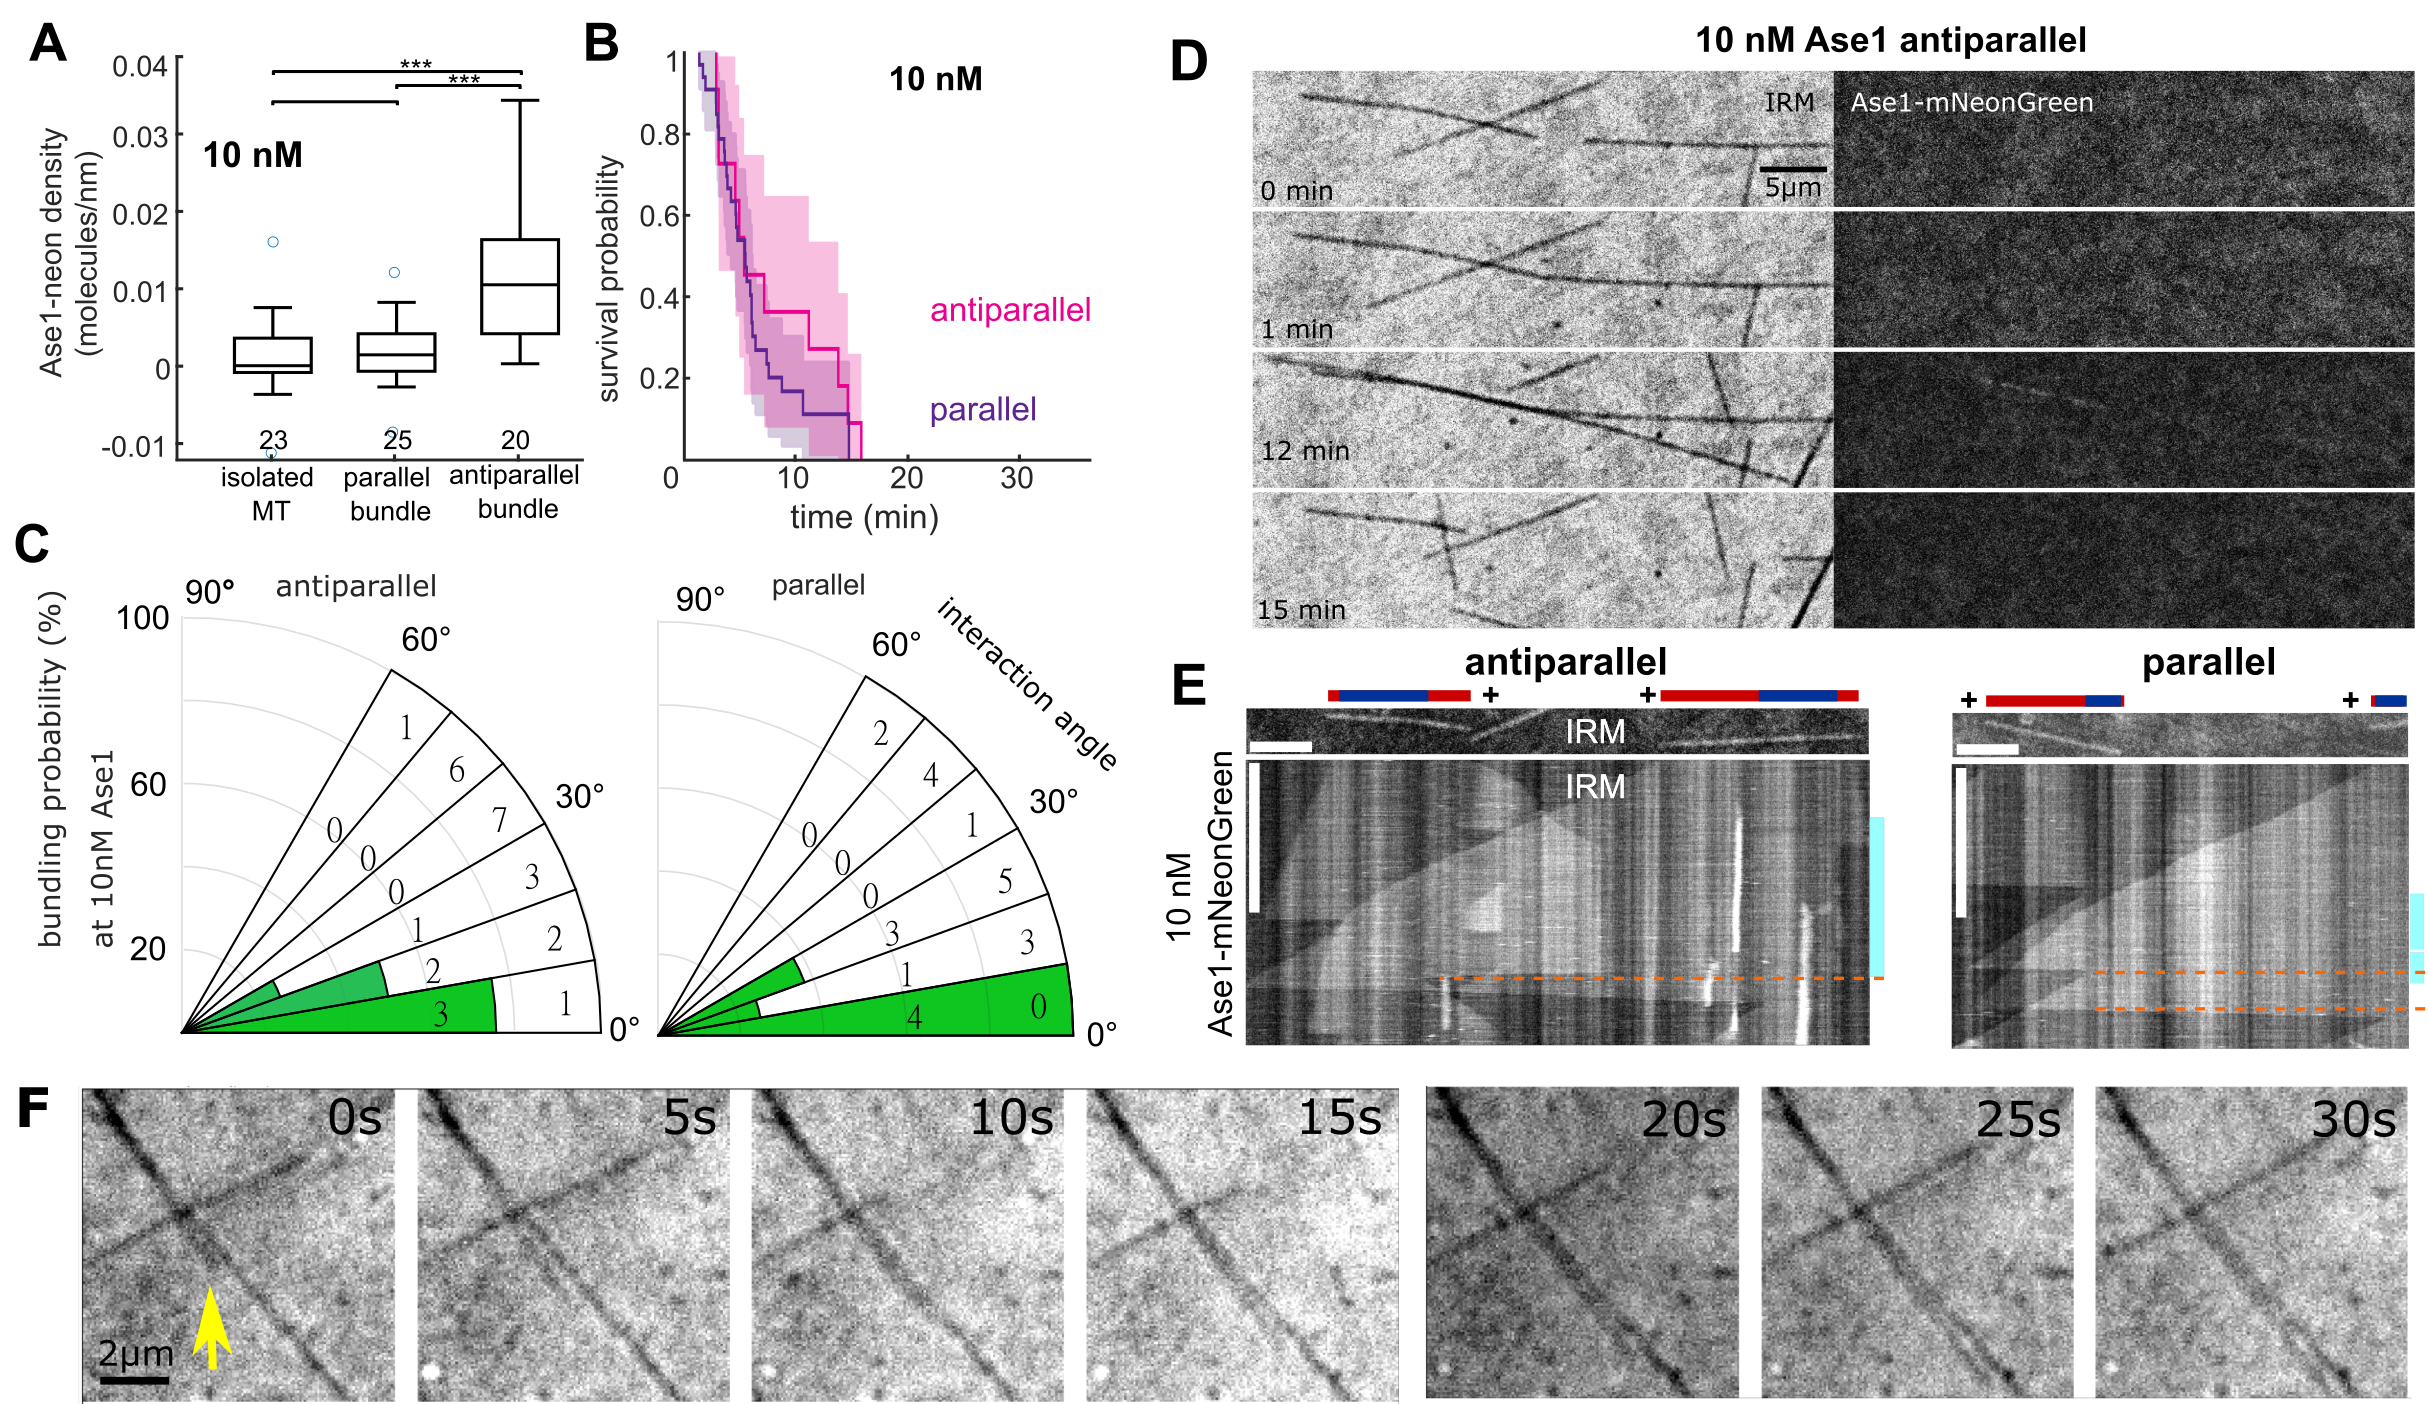
\includegraphics[width=1\linewidth]{Figures/ase1_1c.png}
    \caption[Antiparallel overlaps are not significantly stabilized at low Ase1 concentrations.]{
        (A,B) Quantifications of Ase1 densities and lifetimes for the 10nM Ase1 condition analogous to panels in \autoref{ase1b}. (C) Quantifications of bundling probabilities for the 10nM Ase1 condition analogous to \autoref{ase1a}D. (D) Snapshots of an antiparallel overlap at 10nM Ase1. (E) Kymographs for the 10nM Ase1 condition, representation analogous to \autoref{ase1a}A. The left panel shows the same event as D. (F) A microtubule polymerizing close to another, parallel microtubule at 0nM Ase1 (imaged with IRM). The tip of microtubule in question is indicated by a yellow arrow. As can be seen, no bundling is occurring despite the fact that the microtubules are very close to each other. Panels taken from \cite{Krattenmacher2024}.
        }\label{ase1c}
\end{figure}

Indeed, as indicated by the kymographs shown in \pref{ase1d}{A}, we found rescue frequencies to be increased for antiparallelly crosslinked microtubules at the Ase1 concentrations where we had observed increased lifetimes of these overlaps \pref{ase1d}{B}. To test whether Ase1 crosslinking might have other significant effects on MT polymerization, we next quantified the other three parameters of microtubule dynamic instability. We found that catastrophe frequencies were similar across the tested conditions, with no statistically significant difference between the different populations \pref{ase1d}{C}. Polymerization velocities were similar for all microtubule types, either isolated or bundled, across all tested Ase1 concentrations as well \pref{ase1d}{D}. However, at 420nM Ase1, MTs depolymerized markedly slower than at lower Ase1 concentrations. Further, at 42nM and 420nM Ase1, antiparallel MTs displayed a marked decrease in depolymerization velocity compared to isolated and parallel MTs \pref{ase1d}{E}. Thus, we observed Ase1 to only have a measurable effect on MT depolymerization, by reducing the rate of depolymerization and increasing chances for rescue, with no effect on polymerization.\par

If one only considers our results at 42nM, one could speculate that the particularly pronounced stabilization of antiparallel microtubules was due to the increased number of Ase1 molecules on antiparallel MTs as compared to parallel and isolated MTs. However, at 420nM, the number of Ase1 molecules per MT was similar across all types of MTs, while the antiparallel MTs still were more stable, despite indistinguishable Ase1 densities on antiparallel versus parallel MT overlaps \pref{ase1d}{F,G}. Thus, Ase1 engaged in antiparallel crosslinking seems to have a stronger effect on MT depolymerization than Ase1 engaged in parallel crosslinking or Ase1 not engaged in crosslinking. This deduction is supported by the fact that the number of Ase1 molecules engaged in Ase1 crosslinking was the only factor we could identify as influencing the frequency of rescues (note, however, that the number of molecules directly participating in the crosslinking process, i.e. simultaneously bound to both crosslinked microtubules, is not measurable in this assay). Notably, we with a different set of experiments ("Set B experiments," see Methods) found the same result \autoref{ase1e}, showing the robustness of this finding: At these conditions, we observed antiparallely linked microtubules to exhibit rescues, at a density of around 0.2 molecules per nm which we at these buffer conditions had established with 1nM Ase1 \pref{ase1e}{B,C} (as a side note, the Ase1 used in these experiments had a different fluorescence label, GFP instead of mNeonGreen). At these buffer conditions, isolated microtubules did not exhibit any rescues at all, even when we increased the Ase1 concentration from 1 to 6nM such that the Ase1 density on isolated microtubules was comparable to the Ase1 density on antiparallel bundles at 1nM Ase1 \pref{ase1e}{B,C}. The depolymerization velocity similarly decreased with increasing Ase1 concentration \pref{ase1e}{D}. Altogether, these results show that Ase1 can stabilize antiparallel microtubules while only having minor stabilization effects on MTs outside of such overlaps.

\begin{figure}[h]
    \centering
    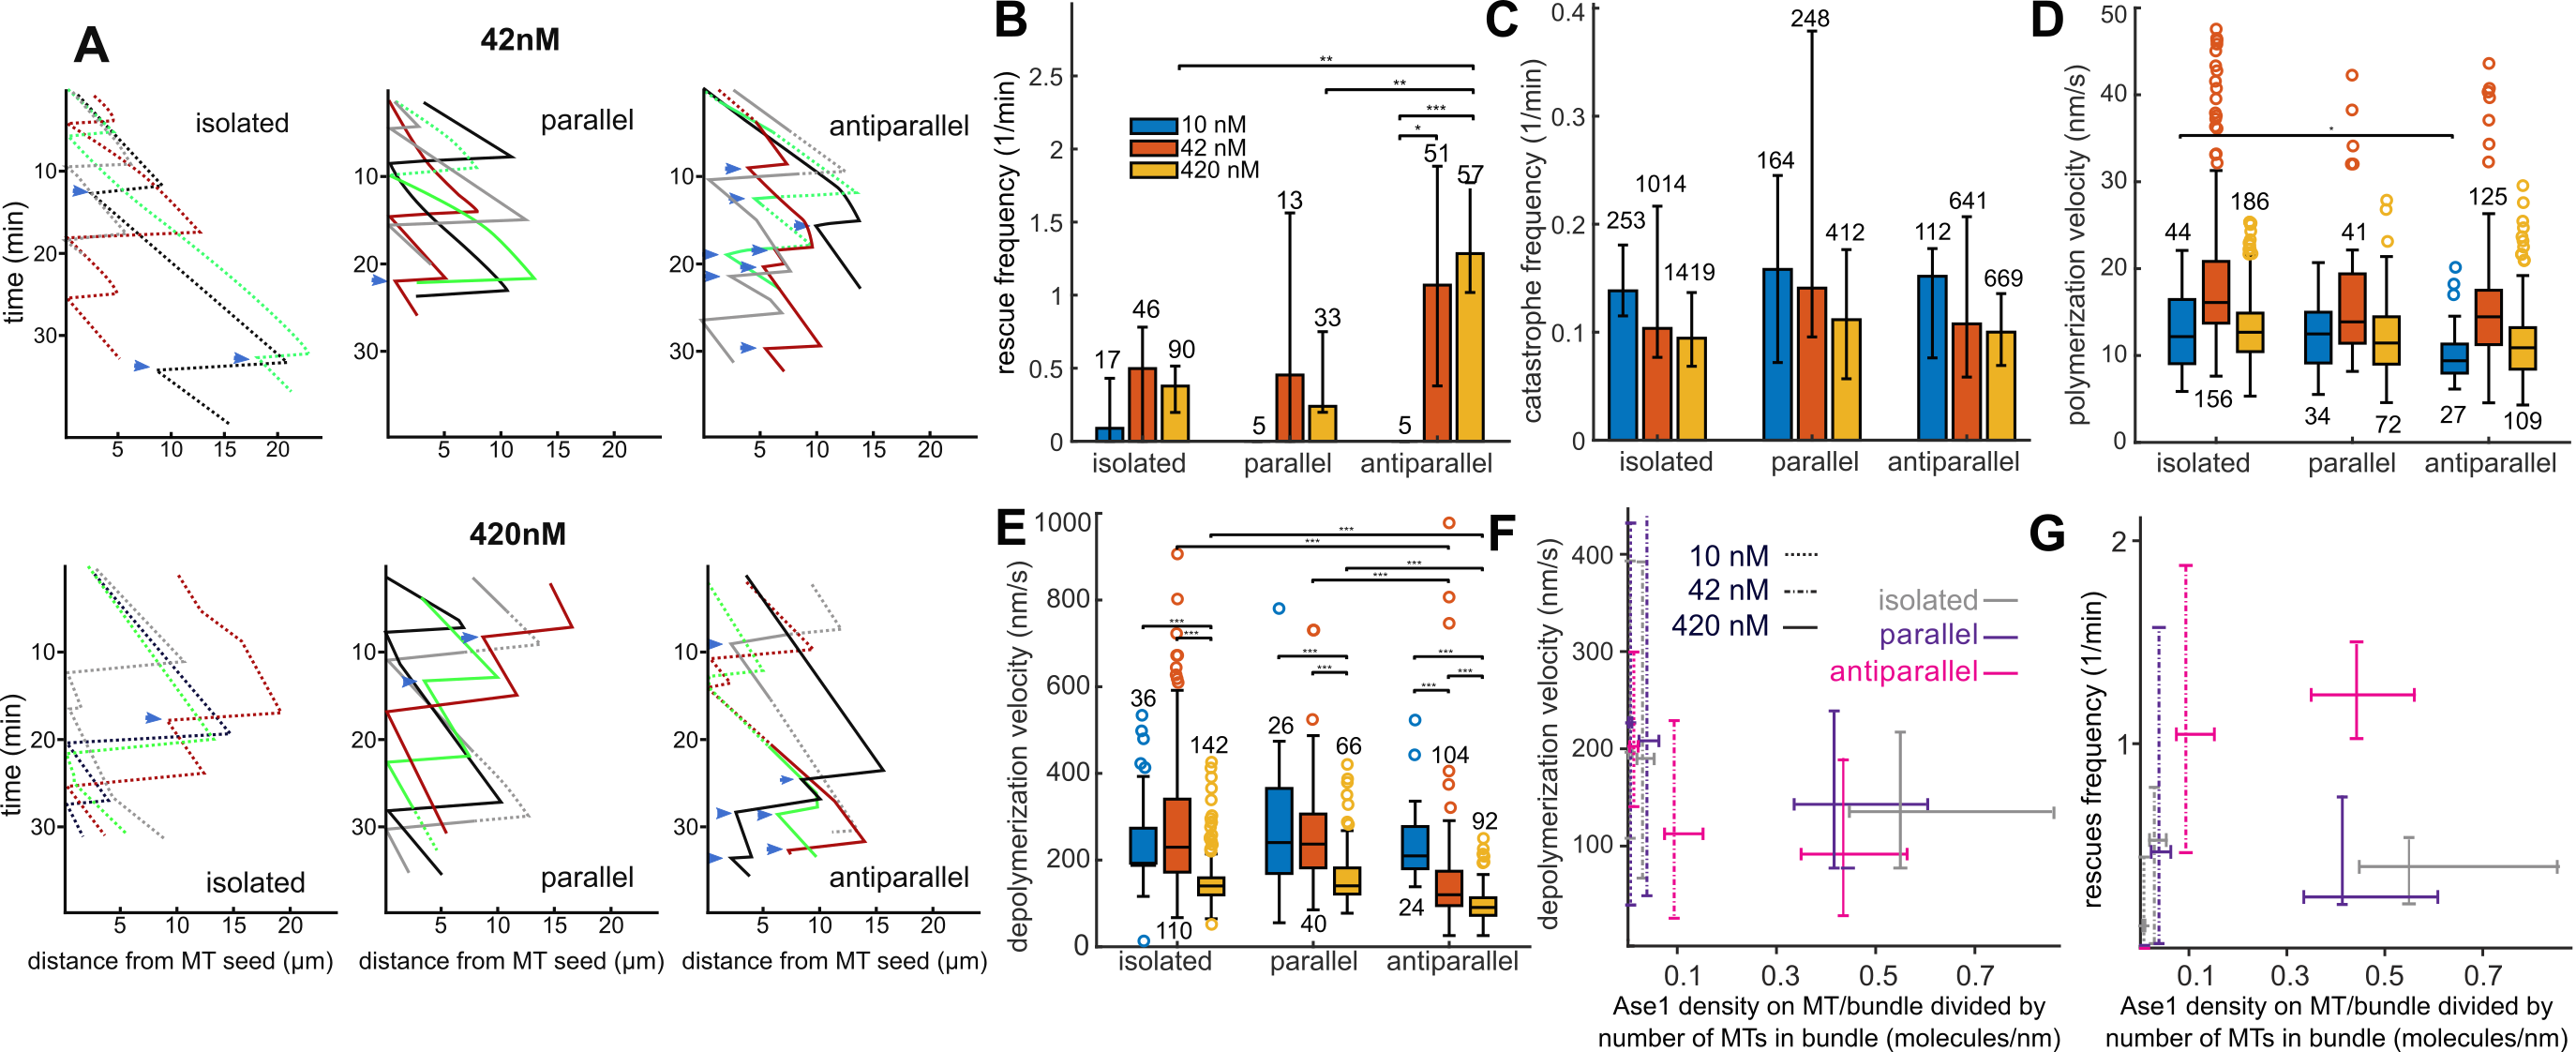
\includegraphics[width=1\linewidth]{Figures/ase1_1d.png}
    \caption[Representative kymograph traces.]{
    (A) Representative kymograph traces of the types of events we observed in our dataset which we present in \autoref{ase1a}, \autoref{ase1b} and \autoref{ase1c}A-E. Blue arrows indicate rescue events. Dotted lines indicate stretches where the MT was isolated. (B) Rescue frequency, (C) catastrophe frequency, (D) polymerization velocity, and (E) depolymerization velocity of dynamic MT plus ends in different configurations and in the presence of varying concentrations of Ase1-mNeonGreen. (F) Depolymerization velocity (see E) versus Ase1-mNeonGreen density on a given MT or bundle divided by number of MTs in that bundle (i.e., the density as shown in \autoref{ase1b}B is divided by 2 in the case of parallel and antiparallel MTs).  (G) Rescue frequency (see B) versus Ase1-mNeonGreen density (see \autoref{ase1b}B). All plots show results for the same experiments as shown in \autoref{ase1a} and \autoref{ase1b}. * p<0.05, ** p<0.01, *** p<0.001 (Tukey's test; only significance levels are visualized that share either the same MT type or the same concentration. No visual link between two populations sharing one such characteristic signifies  p>0.05. In B and C a given population comprises the frequencies recorded for the respective experiments, in D and E the velocities recorded for respective sampled periods). Boxplots are weighted by the length of a sampled period of polymerization or depolymerization. In boxplots, the numbers indicate the number of recorded events, in bar plots, the numbers indicate the sum of the length of all sampled periods of polymerization or depolymerization (in minutes). In bar plots, the height of the bar indicates the catastrophe/rescue frequency as determined from all time lapses (number of total events divided by total duration of depolymerization), while the error bars indicate the lowest and highest rates as determined from each isolated time lapse; velocities are normalized to the median velocity of isolated MTs (Methods). Panels taken from \cite{Krattenmacher2024}.
        }\label{ase1d}
\end{figure}

\begin{figure}[h]
    \centering
    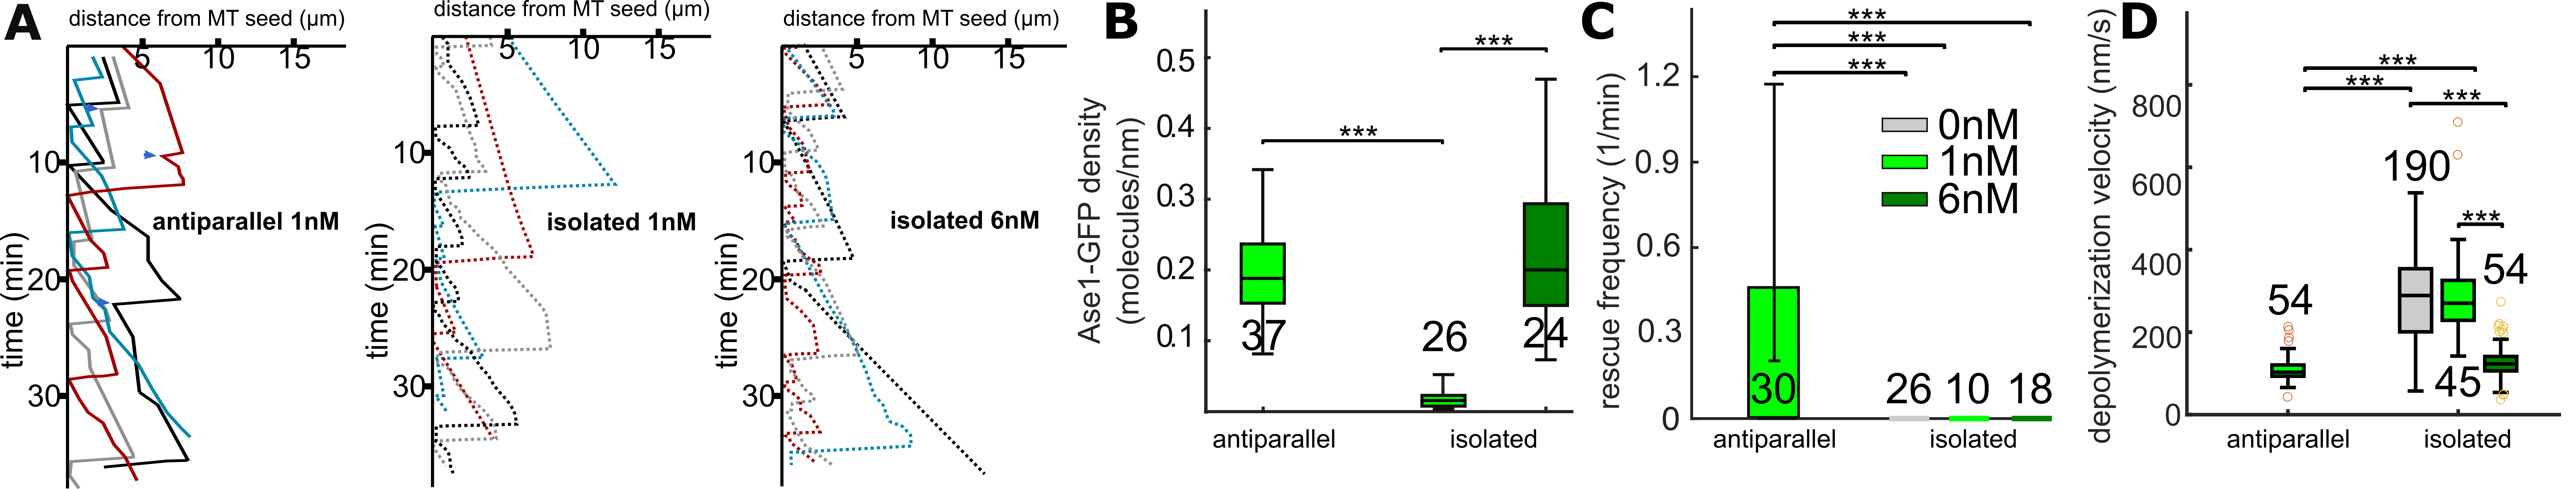
\includegraphics[width=1\linewidth]{Figures/ase1_1e.png}
    \caption[Set B experiments microtubule dynamics.]{
    Data obtained from a second set of experiments ("Set B experiments", see Methods) with different experimental parameters than the data from the set of experiments shown thus far ("Set A experiments"). (A) Representative kymograph traces, representation analogous to \aref{ase1d}{A}. (B) Quantification of the density of Ase1-GFP(Methods). The numbers below the boxes denote the number of analyzed microtubule bundles. (C) Rescue frequency and (D) depolymerization velocity, representations analogous to \aref{ase1d}{B,E}. Legend for B-D in C, showing the concentration of Ase1-GFP in each set of experiments. Panels taken from \cite{Krattenmacher2024}, except panels C and D, which I created only for this thesis.
        }\label{ase1e}
\end{figure}

\FloatBarrier
\subsection{Interactions between Ase1 and the depolymerizing microtubule end}
\label{sec:ase12}
\begin{figure}[h]
    \centering
    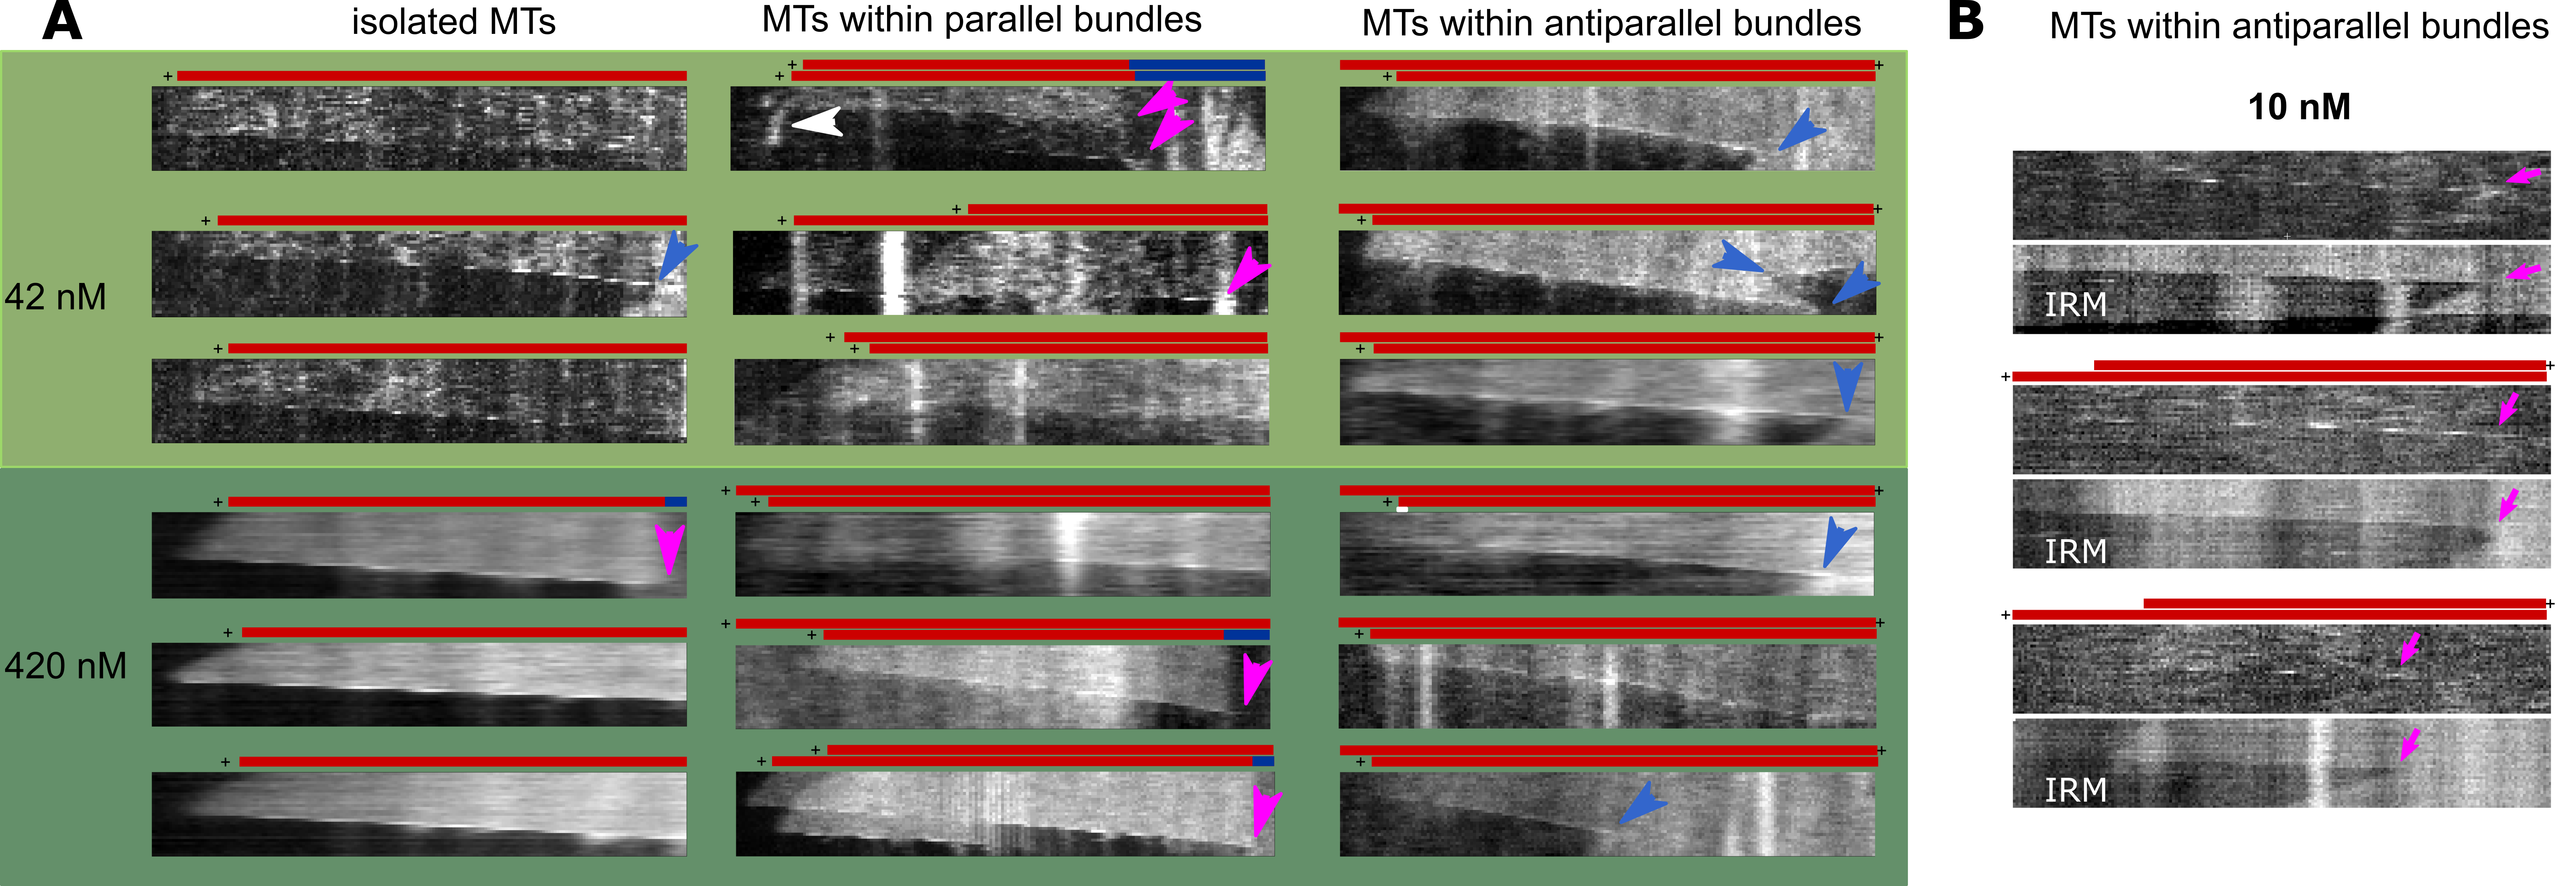
\includegraphics[width=1\linewidth]{Figures/ase2a.png}
    \caption[Set A experiments kymographs showing Ase1 herding.]{Kymographs of depolymerization events (Set A experiments as shown in \aref{ase1d}{A}). (A) Kymographs of all examined microtubule configurations at 42nM and 420nM Ase1. (B) Kymographs of events observed at 10nM Ase1 (antiparallel overlaps only since at this concentration there was no Ase1-mNeonGreen signal at the ends of parallel overlaps and isolated MTs). Each kymograph is 12 µm in width and 150 seconds in height, contrast and balance varies from panel to panel (each kymograph shows a different MT). To facilitate understanding of the kymographs, rescues are pointed out with blue arrows. Pink arrows indicate a MT tip reaching its GMPCPP seed. The white arrow indicates where one of the parallel MTs, before catastrophing, had briefly engaged in antiparallel crosslinking with another isolated MT. Where no arrows are shown, the MT continues to depolymerize toward the right. Panels taken from \cite{Krattenmacher2024}.
        }\label{ase2a}
\end{figure}
Given that we had shown that Ase1 can stabilize depolymerizing microtubules, we suspected that Ase1 molecules very likely interact directly with depolymerizing MT ends. This is indeed what we found when examining the distribution of Ase1. While Ase1 did show no preference for binding to polymerizing MT ends, the kymographs which we had generated showed that Ase1 accumulated at depolymerizing MT ends, for Set A experiments \pref{ase2a}{A,B} as well as Set B experiments \pref{ase2b}{A}. We now set out to quantify this effect. Because the data for Set B experiments allowed for a more fine-grained analysis due to a higher framerate and a more pronounced accumulation effect, we in the following limited our analysis to the Set B experimental data. Given that isolated and parallel MTs behaved very similarly in our assays (though only in Set A experiments we observed a sufficiently high number of parallel overlaps for a thorough analysis), we also chose to focus on comparing isolated and antiparallel MTs.\par
\begin{figure}[h!]
    \centering
    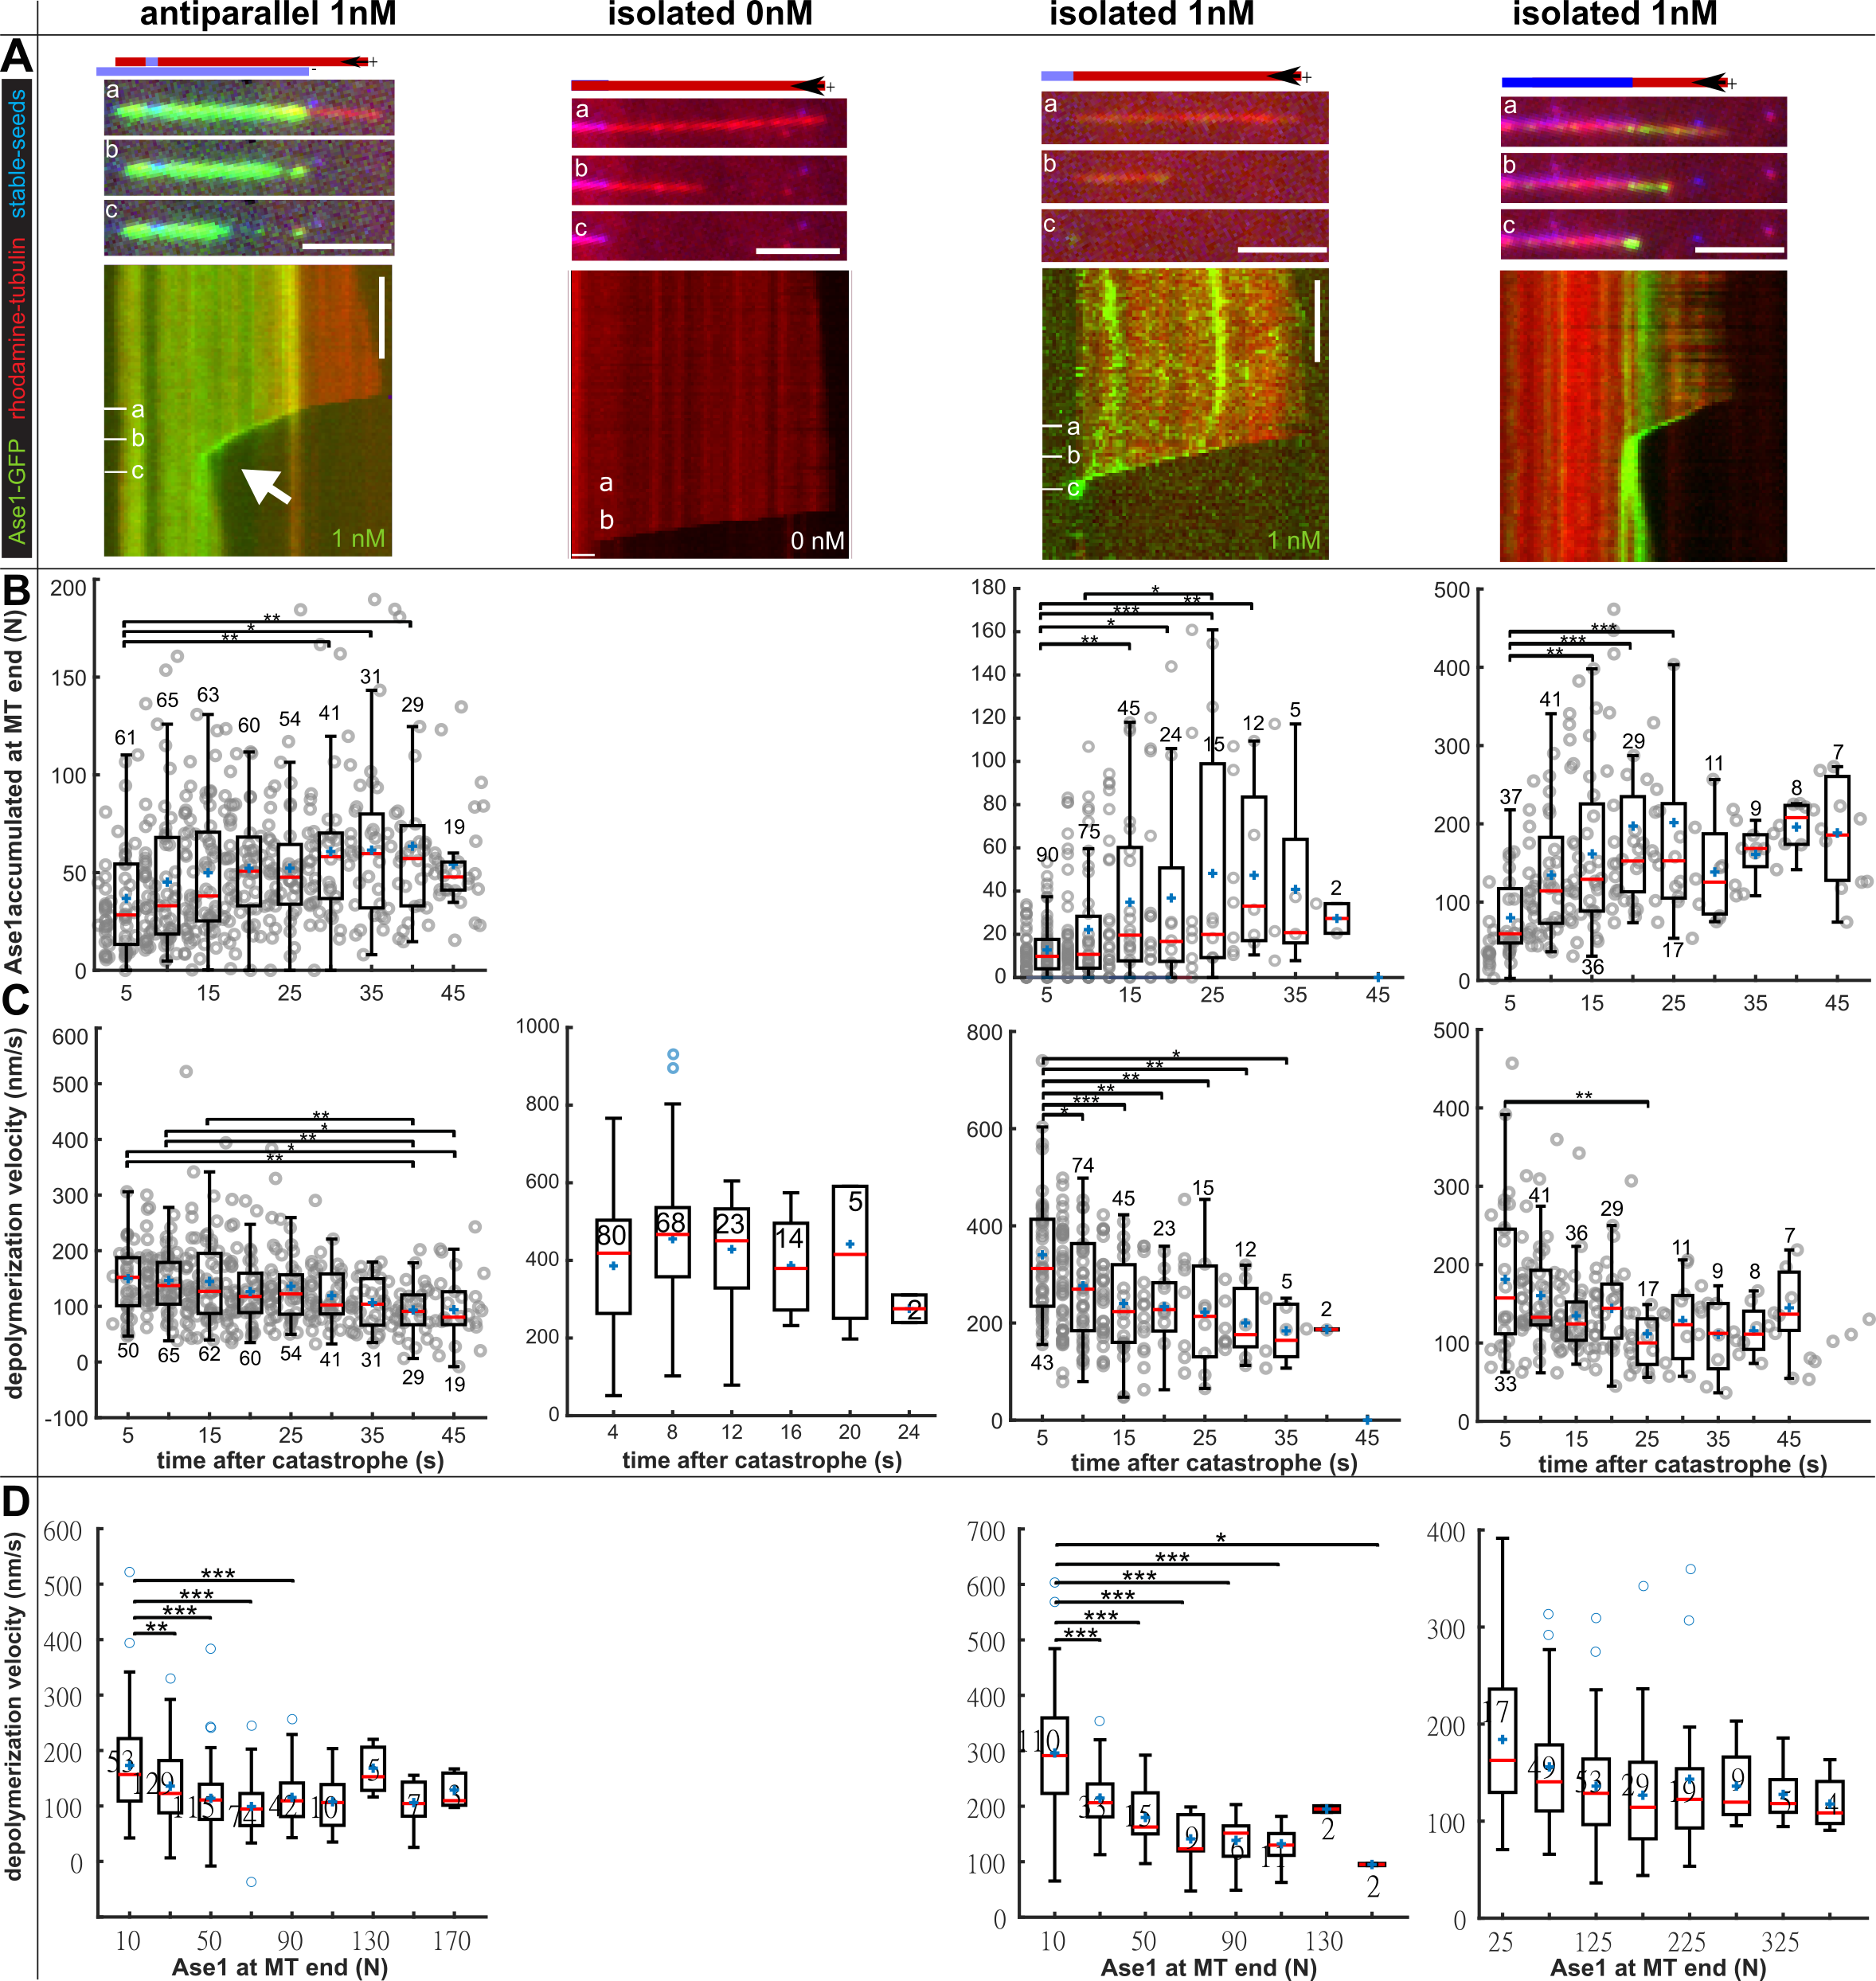
\includegraphics[width=1\linewidth]{Figures/ase2b.png}
    \caption[Ase1 accumulates at depolymerizing MT ends.]{Experimental data on herding of Ase1 (Set B experiments as shown in \aref{ase1e}{A}). (A) Kymographs of depolymerizing MTs. The stabilized GMPCPP-MT seeds were labelled with 15\% rhodamine and 15\% Alexa647 (or, alternatively, with 2\% Alexa647), while the free tubulin in solution was labelled with 7\% rhodamine. In sketches, dynamic extensions with GDP lattices are colored red, and stabilized GMPCPP seeds are colored blue or light blue (in case of the weakly-labelled seeds). The scale bars are 5 micron and 1 minute, contrast and balance vary from panel to panel (each kymograph shows a different MT). White arrows highlight rescue events. (B) The number of additional Ase1 molecules at the end of depolymerizing MTs, plotted over the time passed since the catastrophe. Each data point represents data extracted from one line scan. (C) The frame-to-frame depolymerization velocity of MTs over time (analogous to B). Because the exact time of catastrophe is unknown due to limits in temporal resolution, the velocity measurement right after catastrophe underestimates the actual velocity. (D) Instantaneous depolymerization velocity plotted over number of additional Ase1 molecules at the MT end. Panels taken from \cite{Krattenmacher2024}.
        }\label{ase2b}
\end{figure}

Our quantitative analysis of Ase1 accumulation at depolymerizing microtubule ends confirmed the visual impression given by the kymographs - Ase1 was indeed accumulating at depolymerizing MT ends, for both isolated and antiparallel MTs \pref{ase2b}{B}. In addition, the quantitative analysis also revealed that the Ase1 accumulates were growing the quickest during the early stages of depolymerization \pref{ase2b}{B}. Intuitively, one may expect that this accumulation is related to the stabilization of microtubules during depolymerization. Indeed, Ase1 accumulation correlated with a decrease in depolymerization speed \pref{ase2b}{B-D}. While this correlation does not imply a causal relationship, it does lend support to the existence of such a relationship. An alternative explanation could be a possible hidden third factor, most notably the natural slowdown of depolymerization velocity after catastrophe which has been observed by others \parencite{Luchniak2023}. In other words, it is conceivable that depolymerizing MTs accumulate Ase1 and slow down over time, and that these two phenomena are not causally related. However, in the absence of Ase1 we had not observed any slowdown in MT depolymerization comparable to what we observed in the presence of Ase1 \pref{ase2b}{C}. \par

\begin{figure}[h]
    \centering
    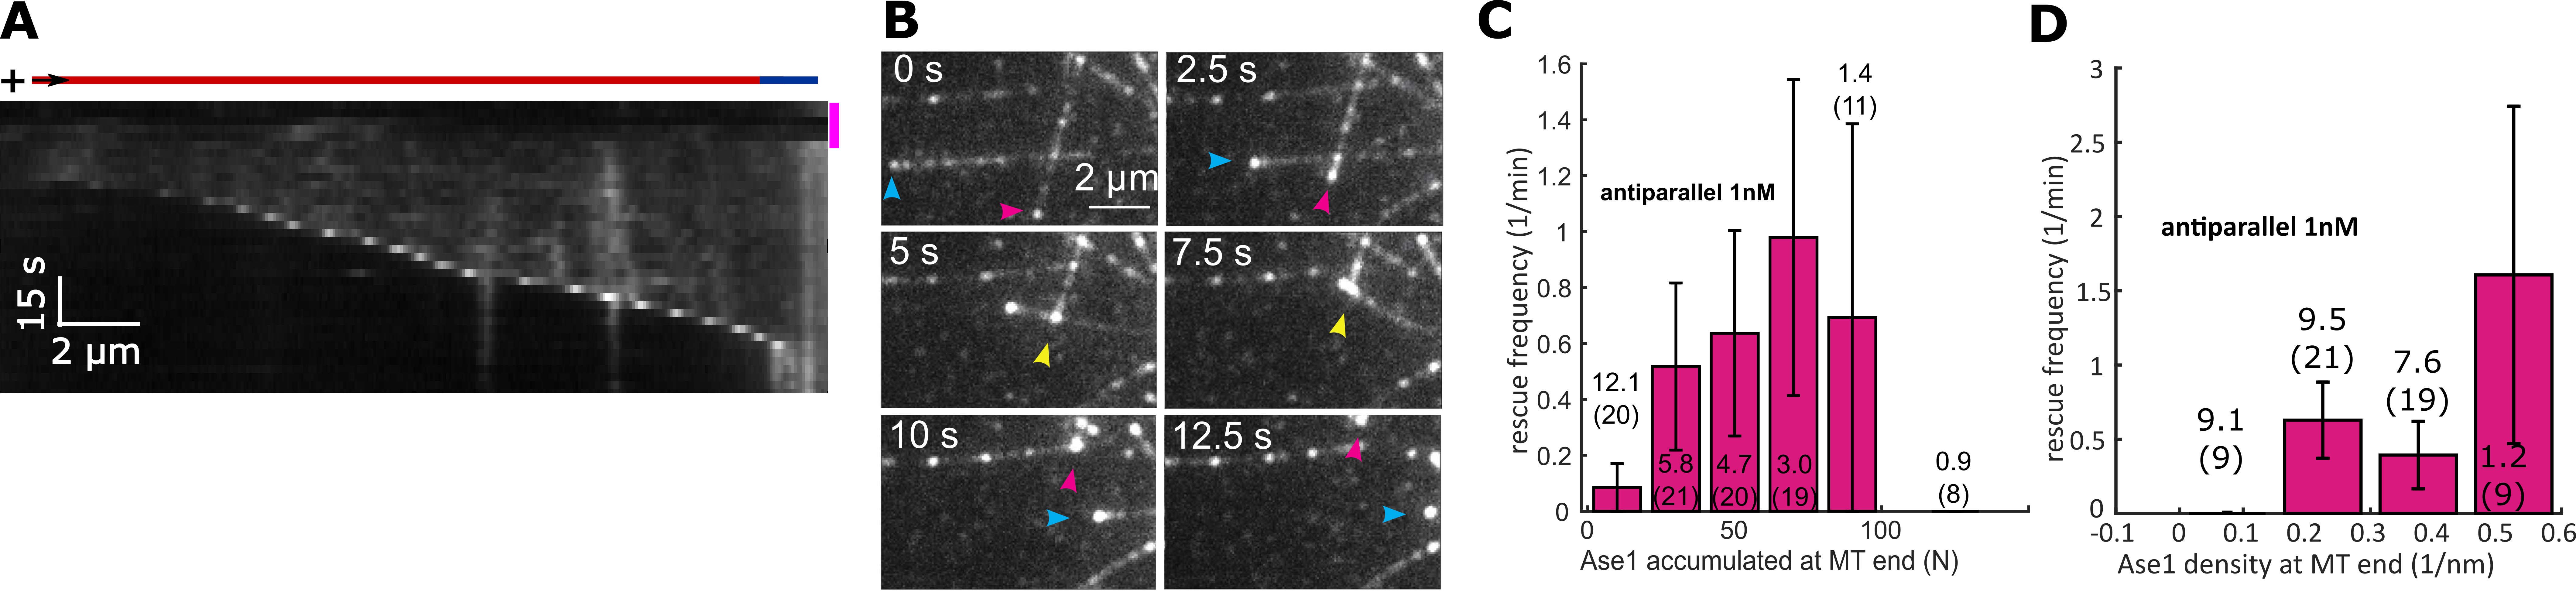
\includegraphics[width=1\linewidth]{Figures/ase2c.png}
    \caption[Ase1 is herded by depolymerizing MTs.]{
    (A) Kymograph (Ase1-mNeonGreen channel) of depolymerizing MT. In this experiment, Ase1 and tubulin had been removed from the assay buffer during the time frame indicated by the pink bar next to the kymograph, prompting subsequent MT depolymerization and concomitant Ase1 accumulation at the end. (B) Time series of micrographs (Ase1-GFP channel) showing an event where the accumulated Ase1 at one depolymerizing MT end (indicated by red arrows) causes the end to “drag” a MT it crosses with it, thereby bending it (yellow arrows). The blue arrows indicate the (depolymerizing) end of the MT before and after it got bent. (C) Rescue frequency plotted over number of additional Ase1 molecules at the MT end. The duration depolymerized at a respective x-value was added to the respective bin. The number of rescues observed in the same bin (N) was then divided by the sum of depolymerization durations (shown in min, the number in parentheses refers to the number of MTs) to estimate the rescue frequency. The correlation coefficient (weighted \parencite{Pelletier2024} by sums of depolymerization durations) is 0.67. The total length of a given error bar equals two times the square root of the number of the rescues in the corresponding bin divided by the sum of the time depolymerized in the corresponding bin. (D) Rescue frequency plotted over the height of the peak of the Ase1 density at the MT end (the weighted correlation coefficient is 0.76). Representation analogous to C. C and D show data from Set B experiments. Panels taken from \cite{Krattenmacher2024}.
        }\label{ase2c}
\end{figure}

Our findings so far suggested that we observed "herding" of Ase1 by the depolymerizing MT end, a phenomenon which has recently been reported for a synthetic MT crosslinker \parencite{Drechsler2019}. To confirm this, we needed to exclude the possibility that Ase1 specifically tracks depolymerizing MT ends by having a higher affinity for depolymerizing MT regions. We thus performed an experiment where we removed both Ase1 and tubulin from solution after first having polymerized Ase1-decorated MTs. We found Ase1 to still accumulate at the ends of depolymerizing MT \pref{ase2c}{A}, indicating that the accumulates are indeed comprised of Ase1 molecules that were already bound to the MT lattice before catastrophe had occurred. As reported for the synthetic polymer \parencite{Drechsler2019}, we also observed instances of depolymerizing MT ends which herded Ase1 molecules pulling on other MTs \pref{ase2c}{B}. This indicates that substantial forces can be transmitted via Ase1 herding.\par

What is the impact of Ase1 herding on the depolymerization of antiparallel MTs in particular? Similarly to what we found in \aref{sec:ase11}{}, we found that the impact of single Ase1 molecules on the depolymerization of antiparallel MTs is stronger than in the case of isolated microtubules: While isolated microtubules at 6nM Ase1 herded more Ase1 than antiparallel microtubules at 1nM Ase1, they did not depolymerize more slowly than antiparallel MTs \pref{ase2b}{B,C}. For antiparallel MTs, we also observed the number of herded Ase1 molecules to positively correlate with the probability of a rescue occuring \pref{ase1c}{C} (a phenomenon we could not test for isolated MTs since they did not exhibit any rescues in this dataset; furthermore, the rescue frequency of isolated MTs appears independent from Ase1 density, see \aref{ase1d}{B}). Moreover, the Ase1 density at the microtubule end, which is a measure for not only accumulated Ase1 but the total number of Ase1 molecules present at the end, also shows a positive correlation with rescue frequency \pref{ase1c}{D}.\par

\begin{figure}[h!]
    \centering
    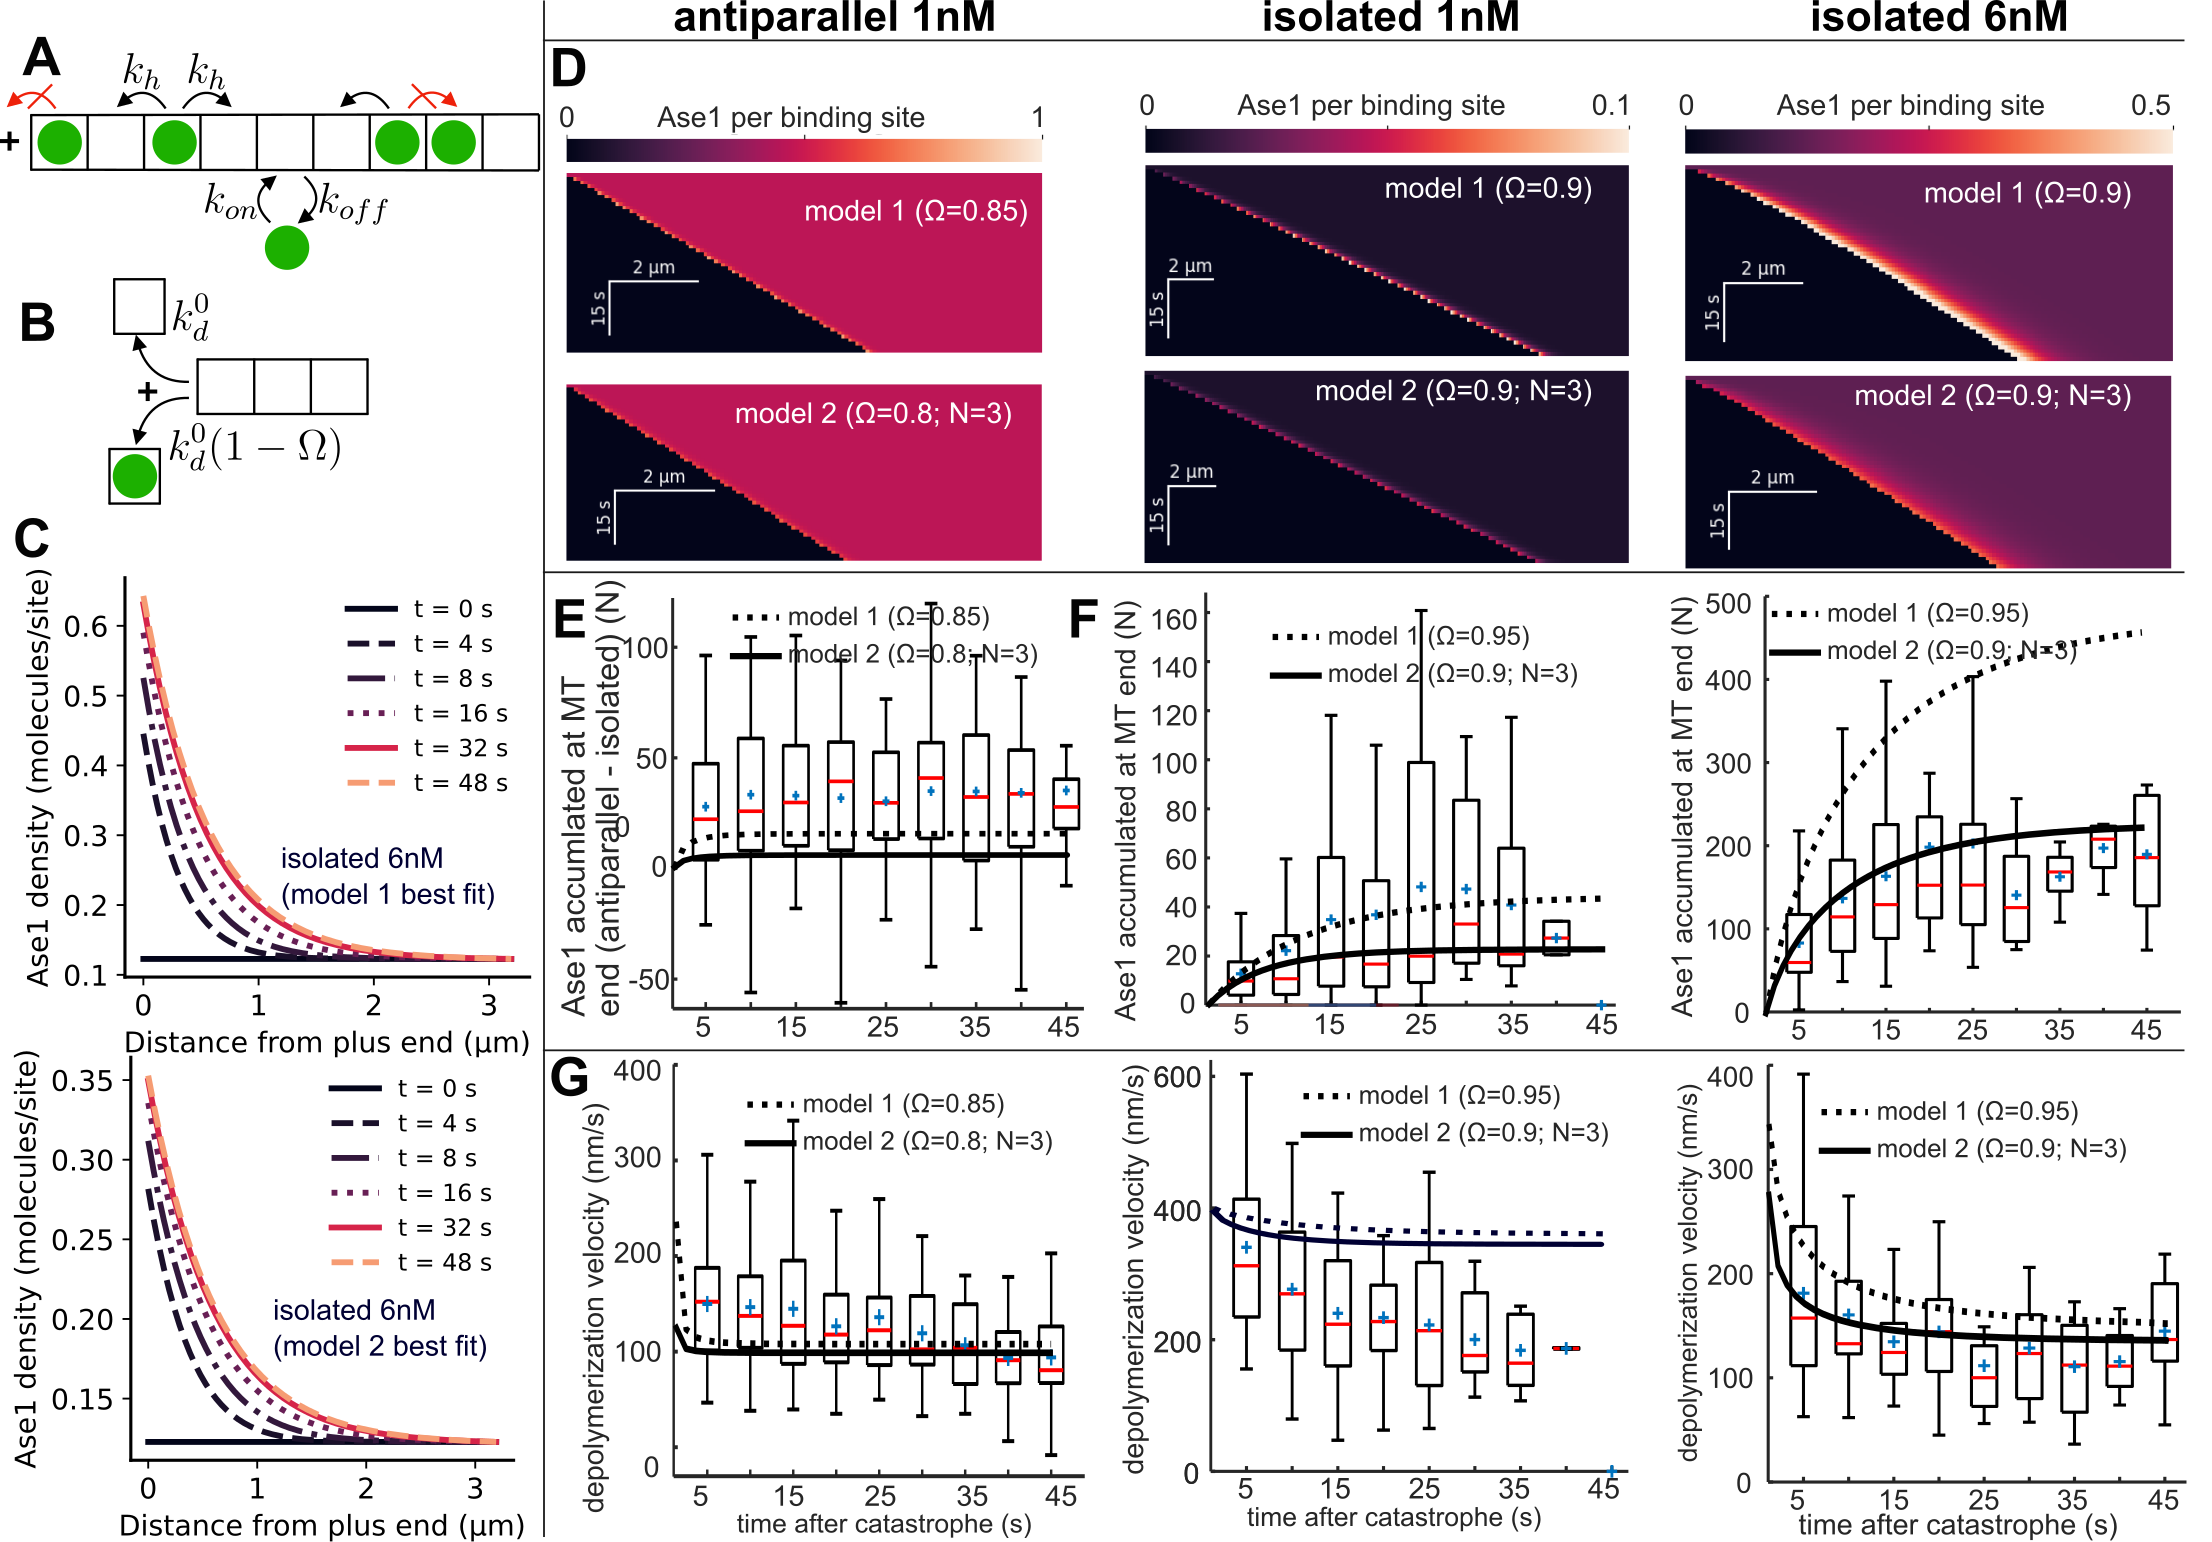
\includegraphics[width=1\linewidth]{Figures/ase2d.png}
    \caption[Modeling of Ase1 herding - results.]{
    (A,B) Cartoons representing model assumptions (see Methods): (A) Ase1 binding, unbind, and hopping to neighboring sites are stochastic events with constant rates $k_{on},k_{off},k_h$. Only one Ase1 molecule can be attached to any one tubulin heterodimer, so moving or binding to an occupied binding site is not allowed (red crossed arrow on the right). Ase1 does not fall off from the MT by hopping at its plus ends (red crossed arrow on the left). (B) In Model 1, we assume that the detachment rate of the tubulin terminal subunit is $k_d^0$ when the first tubulin subunit is free of Ase1, and $k_d=(1-\Omega)k_d^0$ if Ase1 is bound at the terminal site (for Model 2, see Main Text and Methods). (C) Distribution of Ase1 density on terminal sites in time for the indicated timepoints (see legend) as predicted by Model 1 and 2 with model parameters as in F (right panel). $\lambda$, a characteristic x-axis location (see Methods), is visualized for the steady-state curve. (D-G) Modelling results for Model 1 and Model 2 with N=3 (for both models, 3 PFs had been assumed to be engaged in crosslinking in the case of antiparallel MTs, see Methods). Experimental data is presented in the form of boxplots. (D) Distribution of Ase1 density in time represented as a simulated kymograph (see scalebars; in the case of antiparallel MTs, values are for the PFs engaged in crosslinking, the other PFs are assumed to have 0 coverage). (E) Number of crosslinked Ase1 molecules plotted versus time after catastrophe. As an estimate of the number of crosslinked Ase1 molecules, the plot shows the following on the y-axis: The number of additional Ase1 molecules at the end of a depolymerizing antiparallel MT at a given time \pref{ase2b}{B, left panel} minus the median number of additional Ase1 molecules at the ends of isolated MTs in the same experiment as a given antiparallel MT (at the same time after catastrophe) \pref{ase2b}{B, mid panel}. (F,G) Values of Ase1 accumulation and depolymerization velocity derived from experiments (boxplots) or predicted by Model 1 and 2 (lines). The boxplots in F and G are the same as in the corresponding plots in \aref{ase2b}{}. Panels taken or slightly adapted from \cite{Krattenmacher2024}.
        }\label{ase2d}
\end{figure}

\begin{wrapfigure}{l}{0.35\textwidth}
    \centering
    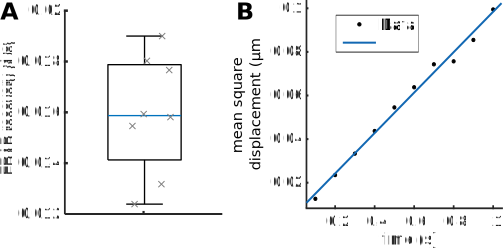
\includegraphics[width=1\linewidth]{Figures/ase2FRAP.png}
    \caption[Experimental determination of the diffusion coefficient and off-rate of Ase1.]{
    (A) Recorded FRAP recovery times on isolated MTs (see Methods) – the median value was used as $k_{off}$ for modelling. (B) Mean square displacement of single Ase1 molecules diffusing on isolated MTs during the first second of their interaction with the MT (see Methods) and fitted line – the slope of the fitted line $D$ was used for modeling ($kh = Da^2$, with $a$ being the tubulin dimer length) (number of molecules = 2008). Panels taken from \cite{Krattenmacher2024}.
        }\label{ase2FRAP}
\end{wrapfigure}

Our experiments thus demonstrate that lattice-bound Ase1 molecules are herded by the depolymerizing MT ends and that the number of swept Ase1 molecules correlates with reduced depolymerization. Yet how do these effects relate to each other? We set out to tackle this question by mathematically modeling Ase1 herding, focusing on the relation between depolymerization velocity and Ase1 accumulation. We thus developed a simple mathematical model that considers a one-dimensional MT made of lattice sites corresponding to tubulin heterodimers, starting at the plus end (see Methods). The model neglects the interaction between protofilaments, and for simplicity focuses on the effect of Ase1 on the depolymerization velocity of isolated MTs. Events such as Ase1 binding, unbinding, and hopping to neighboring sites are stochastic with constant rates $k_{on},k_{off},k_h$ \pref{ase1d}{A}. These rates were determined experimentally, via velocity measurements of depolymerizing MTs under the absence of Ase1 \pref{ase2b}{C, mid panel}, fluorescence recovery after photobleaching (FRAP) experiments \pref{ase2FRAP}{A} and tracking of single Ase1 molecules diffusing on isolated MTs \pref{ase2FRAP}{B}. Importantly, in the model, only one Ase1 molecule can be attached to any one tubulin heterodimer, and Ase1 can thus only hop to unoccupied neighboring sites. We also assume that Ase1 does not fall off from the MT by hopping at its plus ends, as shown experimentally \parencite{Braun2011}. MT depolymerization is modelled stochastically by detachment of the terminal subunit, at a rate that is affected by Ase1 \pref{ase1d}{B}. Specifically, this rate is $k_d^0$ when the first tubulin subunit is free of Ase1, and $k_d=(1-\Omega)k_d^0$, if Ase1 is bound at the terminal site. The value of $k_d^0$ is set by the MT depolymerization velocity in the absence of Ase1, measured experimentally \pref{ase2t1}{}. The parameter $\Omega\in[0,1]$ specifies the effect of Ase1 on depolymerization. If $\Omega=0$, Ase1 has no effect, while if $\Omega=1$, the terminal subunit cannot unbind if Ase1 is bound. For any value $\Omega>0$, this simple model leads to an exponentially-declining accumulation of Ase1 near the depolymerizing end \pref{ase2d}{C}. The accumulation occurs because subunits without Ase1 are more likely to be lost at the plus end, so depolymerization increases the density of Ase1 at the depolymerizing end. At steady state, the system can be characterized by the probability $P_1$ of the terminal site to be occupied, and the rate of subunits loss is $k_d=k_d^0 (1-\Omega P_1)$.\par

\begin{table}[!ht]
    \centering
    \begin{tabular}{|l|l|l|l|}
    \hline
    \makecell{Parameter} & \multicolumn{2}{l|}{Value(s)} & Source \\ \hline
    \makecell{MT depolymerization\\ rate at 0 Ase1} & \multicolumn{2}{l|}{rate equivalent of 400 nm/s} & \aref{ase2b}{C, mid panel} \\ \hline
        Ase1 off-rate ($k_{off}$) & \multicolumn{2}{l|}{0.016 s$^{-1}$} & \aref{ase2FRAP}{A} \\ \hline
        \makecell{Ase1 diffusion\\ coefficient,\\ isolated MTs} & \multicolumn{2}{l|}{0.09 µm$^2$/s} & \aref{ase2FRAP}{B} \\ \hline
        \makecell{Ase1 diffusion\\ coefficient,\\ antiparallel MTs} & \multicolumn{2}{l|}{0.011 µm$^2$/s} & \makecell{8 times lower than isolated MTs\\ \parencite{lanskydiffusible2015}} \\ \hline
        \multirow{3}*{Ase1 on-rate ($k_{on}$)} & Isolated 1nM & 0.00012 $s^{-1}$ & \multirow{2}*{\makecell{Calculated from experimentally\\ measured $k_{off}$ and equilibrium\\ density on MT body\pref{ase1e}{B}}} \\ \cline{2-3}
         & Isolated 6nM & 0.00224 s$^{-1}$ &  \\ \cline{2-3}
         & Antiparallel (3 protofilaments) & 0.01369 s$^{-1}$ &  \\ \hline
         \makecell{Tubulin\\ dimer/binding site\\ length ($a$)} & \multicolumn{2}{l|}{8nm} & \cite{Song1995} \\ \hline
    \end{tabular}
    \caption[Model parameters that are experimentally constrained.]{Model parameters that are experimentally constrained.}\label{ase2t1}
\end{table}

\begin{table}[!ht]
    \centering
    \begin{tabular}{|l|l|l|l|}
    \hline
        Measurement & \multicolumn{2}{l|}{Value and 95\% confidence interval} & Source \\ \hline
        \multirow{3}*{\makecell{Timescale of\\ accumulation ($\tau$)}} & Isolated 1nM & 6.1 s [3.5 s, 11.4 s] & \multirow{6}*{\makecell{Fit of data shown\\ in \aref{ase2d}{E,F}\\ to\\ $A_{end}(1-e^{-t/\tau})$}} \\ \cline{2-3}
         & Isolated 6nM & 7.2 s [5.5 s, 11.4 s] &  \\ \cline{2-3}
         & Antiparallel & 2.4 s [1.2 s, 4.9 s] &  \\ \cline{1-3}
        \multirow{3}*{\makecell{Molecules accumulated\\ at steady state,\\ per MT ($A_{end}$)}}  & Isolated 1nM & 22 [17, 29] &  \\ \cline{2-3}
         & Isolated 6nM & 185 [160, 247] &  \\ \cline{2-3}
         & Antiparallel & 31 [24, 41] &  \\ \cline{1-4}
        \multirow{3}*{\makecell{Depolymerization\\ velocity at\\ steady state}} & Isolated 1nM & 226 nm/s [194 nms/s, 254 nm/s] & \multirow{3}*{\makecell{Average value after\\ 20 seconds of\\ depolymerization}} \\ \cline{2-3}
         & Isolated 6nM & 137 nm/s [122 nm/s, 151 nm/s] &  \\ \cline{2-3}
         & Antiparallel & 117 nm/s [108 nm/s, 125 nm/s] &  \\ \hline
    \end{tabular}
    \caption[Experimental measurements that are compared with model predictions.]{Experimental measurements that are compared with model predictions. Confidence intervals (95\%) are calculated with the bootstrap method (see Methods).}\label{ase2t2}
\end{table}

All parameters of this model (Model 1) were set from experimental measurements except for $\Omega$. Therefore, we tested whether any value of $\Omega$ could quantitatively recapitulate the experimental behavior of isolated MTs. We chose to focus on the 6nM Ase1 condition, as the case of antiparallel MTs is structurally more complex (see Discussion), and as our mean field approach may not be suitable for the low Ase1 densities we observed for isolated MTs at the 1nM Ase1 condition. Specifically, we aimed to reproduce the timescale of accumulation of Ase1, and the total amount of Ase1 accumulated and depolymerizing velocity reached at steady state \pref{ase2t2}{}. For $\Omega=0.95$, the model predicted depolymerization velocities comparable to the ones observed experimentally \pref{ase1d}{G, right panel}, but the timescale and number of Ase1 molecules accumulated at steady state were respectively two and three times higher than experimentally observed \pref{ase1d}{F, right panel}. Therefore, despite recapitulating the experimental phenomenology qualitatively \pref{ase1d}{D, right panel}, this first model was insufficient to quantitatively reproduce our experimental results.\par

The failure of Model 1 indicated that Ase1 should affect MT depolymerization at lower density. We thus hypothesized that Ase1 molecules located at lattice sites other than the terminal one could affect depolymerization.\footnote{This hypothesis, and the preliminary modeling of it, were my main contribution to the modeling part of our publication.} Therefore, we tested the possibility that the rate of tubulin subunits loss at the plus end would be reduced by a factor $(1-\Omega)$ if any of the N terminal sites were occupied. This rate at steady state would then be $k_d=k_0^d [1-\Omega{1-\prod_{i=1}^{i=N}(1-P_i)}]$, where $P_i$ is the probability of site i being occupied by Ase1. N is not experimentally constrained, but the range of possible values is small, since it is unlikely that distant tubulin subunits could affect the detachment of the terminal subunit. For $N=3$ and $\Omega=0.9$ this model (Model 2) recapitulated the dynamics of the system \pref{ase2d}{F,G, right panels} and reproduced MT depolymerization velocity and Ase1 accumulation at steady state and Ase1 accumulation timescale \pref{ase2steady}{}. The model predicts that at steady state Ase1 density should decay exponentially from the plus end with a length scale of around 600nm \pref{ase2d}{C}. Experimentally, we observed a decay of Ase1 signal from the plus end with length scale of around 200 nm \pref{ase2e}{A}. However, this signal is hardly comparable with our isolated-protofilament model, not only because it comes from multiple protofilaments that may not be in register, but also because shrinking protofilaments are likely curved outwards \parencite{McIntosh2008}.\par

\begin{wrapfigure}{l}{0.45\textwidth}
    \centering
    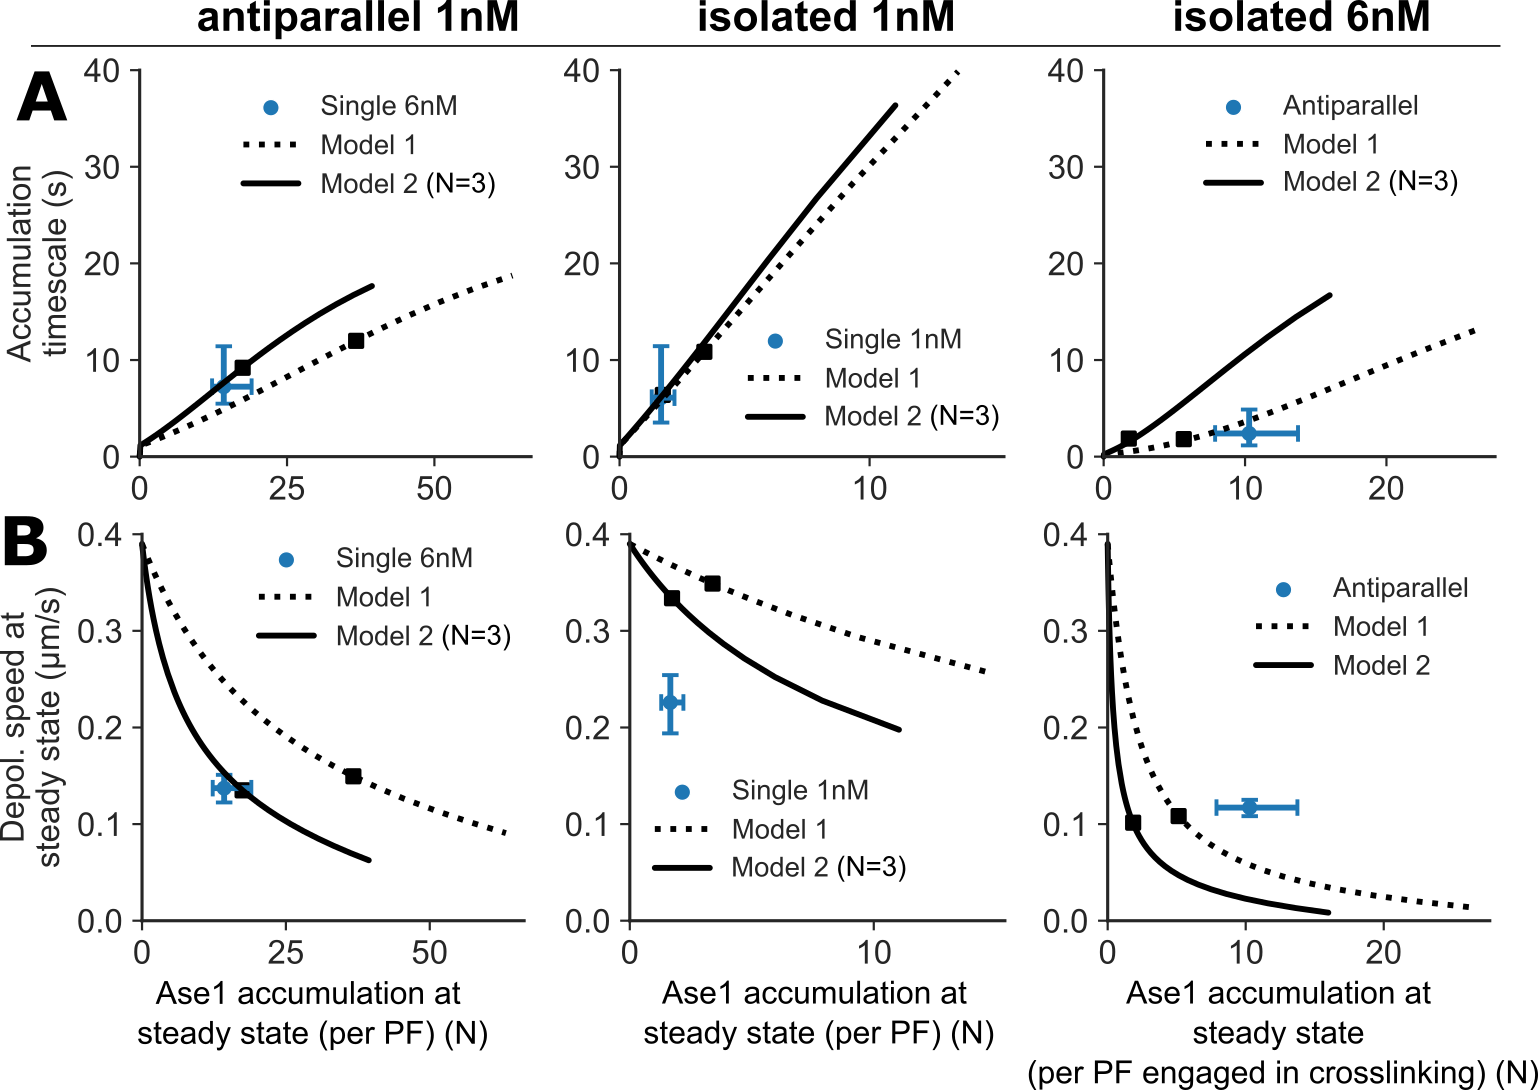
\includegraphics[width=1\linewidth]{Figures/ase2steady.png}
    \caption[Steady-state analysis of the mathematical models.]{
        (A) Values of depolymerization velocity and Ase1 accumulation at steady state derived from experiments (blue dot) or predicted by Model 1 and 2 (lines). Experimental values were derived from the depolymerization events shown in Figure 3, and the error bars represent 95\% confidence intervals calculated using the bootstrap method (see \aref{ase2t2}{} and Methods). The lines represent all the solutions of each model from $\Omega = 0$ to $\Omega = 1$, with $N = 3$ for Model 2. Black squares mark the parameter values of $\Omega$ that best fit the experimental data: Model 1 with $\Omega = 0.95$ and Model 2 with $\Omega = 0.9$ for isolated MTs (assuming 13 PFs), and Model 1 with $\Omega = 0.85$ and Model 2 with $\Omega = 0.8$ for antiparallel overlaps (assuming 3 crosslinking PFs). PF = Protofilament. (B) Same as A, with accumulation timescale in the x axis. 
    }\label{ase2steady}
\end{wrapfigure}

Using Model 2 with the same value of $\Omega=0.9$, we could recapitulate the Ase1 accumulation timescale and steady state accumulation in isolated MTs with 1nM of Ase1 \pref{ase2d}{F}, but the model predicted a ~15\% decrease with respect to the maximum velocity while the experimentally observed decrease was between 35\% and 50\% (\aref{ase2d}{G}, \aref{ase2t2}{}). The reason for this disagreement is likely the low density of Ase1 molecules at 1nM concentration (<1\% of tubulin dimers bound to Ase1 in the body of isolated MTs vs. ~12\% at 6nM of Ase1). At this very low density, the stochasticity of the system may not be well captured by our mean field approach (see Methods). The model also fails to reproduce the behavior of antiparallel overlaps (\aref{ase2d}{E,G left panel}, \aref{ase2steady}{left panels}). This is not surprising given that overlaps are not symmetric, and some protofilaments have almost no Ase1, while others have extremely high Ase1 density (76\% tubulin dimers bound to Ase1 in the MT body assuming 2 protofilaments crosslinked, 50\% assuming 3, see “Mathematical modelling” in Methods). A more complex model accounting for protofilament interactions would be needed for overlaps, but it would need to be informed by experimental measurements of such interactions. However, it is also possible that we simply are overestimating the number of Ase1 molecules herded by antiparallel MTs, because part of the Ase1 which is lost at the depolymerizing MT end presumably remains bound to the template MT, an effect which we do not account for in our estimation. A likely expression of this effect is our observation that while at the ends of isolated MTs, we observed a (blurred) right-sided exponential decay of additional Ase1 density as predicted by our model, the additional Ase1 density at the ends of antiparallel MTs were more reminiscent of a gaussian \pref{ase2e}{B-D}. In particular, the exponential fits often did not fully capture the additional Ase1 density we observed which "lingered" behind the depolymerizing MT end, an additional density which the gaussian fits did capture.\footnote{Because this additional density is likely due to Ase1 molecules still bound to the template MT after detaching from the depolymerizing MT end, we decided to base our analysis as shown in \aref{ase2d}{} on the results stemming from the exponential fits.}\par
In summary, our simple model shows that the necessary assumption that Ase1 prevents depolymerization at plus ends is sufficient to explain sweeping at shrinking microtubule ends without further assumptions. Subunits without Ase1 are more likely to be lost at the plus-end, so depolymerization increases the density of Ase1 at the depolymerizing end. The model recapitulated quantitatively the behaviour of the system for 6nM of Ase1, and within an order of magnitude for 1nM of Ase1. However, a more complicated model may be required to explain the behaviour of MT overlaps.



\begin{figure}[h]
    \centering
    
\includegraphics[width=1\linewidth]{Figures/ase2e.png}
    \caption[Difference between the distribution of Ase1 on antiparallel and isolated MTs.]{
    (A) Fitting results for the lengthscale of the exponential decay $\lambda$ for all fitted density profiles $D_A $(as described in the methods). *** p<0.001 (Tukey's test). (B) An example Ase1 density profile $D_A$ and visualized fitting results for an antiparallel overlap midway during depolymerization. The microtubule seed is on the left, and depolymerization proceeds toward the left. The yellow region shows the fitted region between $X_{Dsleft}$ and $X_{Dsright}$ (Methods). (C) An example Ase1 density profile $D_A$ visualized fitting results for an isolated MT midway during depolymerization (representation analogous to B). (D) The number of accumulated Ase1 molecules as determined by the exponential (plus error function) fit divided by the number of accumulated Ase1 molecules as determined by the gaussian (plus error function) fit (numbers as determined for each respective density profile). Panel A taken from \cite{Krattenmacher2024}, the others I created only for this thesis.
        }\label{ase2e}
\end{figure}